\documentclass[journal]{IEEEtran}
\usepackage{epsf}
\usepackage{filecontents}
\usepackage{times}
\usepackage{amsmath,amssymb}
\usepackage{graphicx}
\usepackage{color}
%\usepackage{subfigure}
\usepackage{cite}
\usepackage{multirow,tabularx}
\usepackage{cases}
\usepackage{ifthen}
%\usepackage[figure]{algorithm2e}
\usepackage{wasysym}
\usepackage{stackrel}
%\usepackage{hyperref}
\usepackage{enumerate}
\usepackage{microtype} 
\usepackage{array}
\usepackage{mathtools}
\usepackage{amsfonts}
\usepackage{bm}
\newcolumntype{L}[1]{>{\raggedright\let\newline\\\arraybackslash\hspace{0pt}}m{#1}}
\newcolumntype{C}[1]{>{\centering\let\newline\\\arraybackslash\hspace{0pt}}m{#1}}
\newcolumntype{R}[1]{>{\raggedleft\let\newline\\\arraybackslash\hspace{0pt}}m{#1}}


\setlength{\skip\footins}{0.6cm}
%------------------
% \include{../../commonHeader}

\newcommand{\hide}[1]{\ifthenelse{\boolean{false}}{#1}{}}
%%%%%%%%%%%%%%%%%%%%%%
% Theorems, etc.

\newtheorem{theorem}{{\bf Theorem}}
\newtheorem{lemma}{{\bf Lemma}}
\newtheorem{proposition}[theorem]{Proposition}
\newtheorem{corollary}{{\bf Corollary}}
\newtheorem{result}{{\bf Result}}

%\newenvironment{proof}[1][Proof]{\begin{trivlist}
%\item[\hskip \labelsep {\bfseries #1}]}{\end{trivlist}}

%\newtheorem{defn}{Definition}
\newenvironment{definition}[1][Definition]{\begin{trivlist}
\item[\hskip \labelsep {\bfseries #1}]}{\end{trivlist}}

\newenvironment{example}[1][Example]{\begin{trivlist}
\item[\hskip \labelsep {\bfseries #1}]}{\end{trivlist}}

\newenvironment{remark}[1][Remark]{\begin{trivlist}
\item[\hskip \labelsep {\bfseries #1}]}{\end{trivlist}}

\newcommand{\qed}{\nobreak \ifvmode \relax \else
      \ifdim\lastskip<1.5em \hskip-\lastskip
      \hskip1.5em plus0em minus0.5em \fi \nobreak
      \vrule height0.75em width0.5em depth0.25em\fi}


\newtheorem{fact}{Fact}
\newtheorem{obs}{Observation}

%%%%%%%%%%%%%%%%%%%%%%
% Environments

\newcommand{\barr}{\begin{array}}
\newcommand{\earr}{\end{array}}



%%%%%%%%%%%%%%%%%%%%%%
% References

\newcommand{\eqn}[1]{(\ref{#1})}

%%%%%%%%%%%%%%%%%%%%%%
% Brackets

\newcommand{\brac}[1]{\left({#1}\right)}
\newcommand{\sbrac}[1]{\left[{#1}\right]}
\newcommand{\cbrac}[1]{\left\{{#1}\right\}}

\newcommand{\floor}[1]{\left\lfloor{#1}\right\rfloor}

%%%%%%%%%%%%%%%%%%%%%%
% Misc

\newcommand{\expc}[2][]{E_{#1}\left[{#2}\right]}

\newcommand{\set}[1]{\{#1\}}

\newcommand{\ul}{\underline}
\newcommand{\smq}[1]{{\it #1}}
\newcommand{\ave}[1]{\overline{#1}}

\newcommand{\recip}[1]{\frac{1}{{#1}}}

%%%%%%%%%%%%%%%%%%%%%%
% Indicator function

\newcommand{\indic}[1]{I_{\cbrac{#1}}}

%%%%%%%%%%%%%%%%%%%%%%
% Superscripts
\newcommand{\supth}{^{{\mathrm{th}}}}
\newcommand{\mth}{^{{\mathrm{th}}}}
\newcommand{\supnd}{^{{\mathrm{nd}}}}
\newcommand{\suprd}{^{{\mathrm{rd}}}}


%%%%%%%%%%%%%%%%%%%%%%
% Combinatorics

\newcommand{\nchoosek}[2]{\left(\begin{array}{c}
                                {#1} \\ {#2}
                             \end{array}
                        \right)}

%%%%%%%%%%%%%%%%%%%%%%
% Symbols
\newcommand{\CN}{{\cal CN}}
\newcommand{\db}{{\mathrm dB}}
\newcommand{\Om}{\widehat{\Omega}}

\newcommand{\define}{\triangleq}
%\newcommand{\define}{\stackrel{\triangle}{=}}
%\newcommand{\implies}{\Rightarrow}
%\newcommand{\tendsto}{\rightarrow}
\newcommand{\tendsto}{\to}

\newcommand{\degree}{^{\circ}}
\newcommand{\kroneck}{\otimes}

%%%%%%%%%%%%%%%%%%%%%%
% Special phrases

\newcommand{\ie}{{i.e.}}
\newcommand{\eg}{{e.g.}}
\newcommand{\etal}{{et al.}}
\newcommand{\wrt}{w.r.t.}
\newcommand{\vs}{{vs.}}

%%%%%%%%%%%%%%%%%%%%%%
% Matrix related

\newcommand{\tvec}{\text{vec}} % \vec is already defined
\newcommand{\mtx}[1]{{\bf #1}} % matrix
\newcommand{\mtxg}[1]{{\boldsymbol #1}} % matrix for greek symbol

\newcommand{\trp}{\text{T}} % transpose
\newcommand{\trc}[1]{\text{Tr}\left\{{#1}\right\}} % trace

%%%%%%%%%%%%%%%%%%%%%%
% Special matrices


\newcommand{\mzero}{\mtx{0}}

%%%%%%%%%%%%%%%%%%%%%%
% Principal sub-matrix

\newcommand{\princ}[2]{{#2}^{({#1})}}
\newcommand{\princsup}[3]{{{#2}^{({#1})^{#3}}}}

%%%%%%%%%%%%%%%%%%%%%%
% Probability related

\newcommand{\EX}{\bf{E}} % expectation operator
\newcommand{\expect}[1]{{\bf{E}}\left[{#1}\right]}
\newcommand{\expectpow}[2]{{\bf{E}}^{#2}\left[{#1}\right]}
\newcommand{\explow}[2]{{\bf{E}}_{#1}\left[{#2}\right]}
\newcommand{\prob}[1]{\text{Pr}\brac{#1}}
\newcommand{\pr}{{\text{Pr}}}

%%%%%%%%%%%%%%%%%%%%%%
% Derivatives

\newcommand{\deriv}[2]{\frac{d{#1}}{d{#2}}}
\newcommand{\pderiv}[2]{\frac{\partial{#1}}{\partial{#2}}}

%%%%%%%%%%%%%%%%%%%%%%
% Slides

\newcommand{\bsp}{\begin{slide*}}
\newcommand{\esp}{\end{slide*}}
\newcommand{\bsl}{\begin{slide}}
\newcommand{\esl}{\end{slide}}
\newcommand{\vsp}[1]{\vspace{#1}}





%-------------------------------
% This paper's specific shortcuts

\newcommand{\nbm}[1]{{[\bf nbm: #1]}}
\newcommand{\vinod}[1]{[\textsl{v: #1}]}
\newcommand{\var}[1]{{\bf var}\left[{#1}\right]}
\newcommand{\opt}{\text{opt}}
\newcommand{\sth}{\text{th}}

\DeclareMathOperator*{\argmin}{arg\,min}
\DeclareMathOperator*{\argmax}{arg\,max}
%\newcommand{\var}{var}

\newcommand{\dv}{D}
\newcommand{\newdv}{{\cal D}^{\prime}}

\newcommand{\abs}[1]{\left\lvert{#1}\right\lvert}

%\newcommand{\err}{\text{Err}}

\newcommand{\given}{\arrowvert}
\newcommand{\givens}{\big\arrowvert}
\newcommand{\Given}{\Big\arrowvert}

\newcommand{\bMQAM}{b_{\text{QAM}}}
\newcommand{\bMPSK}{b_{\text{PSK}}}

\newcommand{\cMPSK}{c_{\text{PSK}}}
\newcommand{\cMQAM}{c_{\text{QAM}}}

%\newcommand{\opt}{\text{opt}}
%\newcommand{\asym}{\text{asm}}


%\newcommand{\err}{\text{Err}}


%% \newcommand{\alphaoptasm}{\alpha_{\opt}^{\asym}}
%% \newcommand{\betaoptasm}{\beta_{\opt}^{\asym}}


%\newcommand{\sepMPSK}{P_{\text{MPSK}}}

\newcommand{\limgamma}{\lim_{\gamma \tendsto \infty}}


\newcommand{\SEP}{\text{SEP}}
\newcommand{\SEPdouble}{\text{SEP}_{\text{si}}}


\newcommand{\sinpiM}{\sin^2\brac{\frac{\pi}{M}}}

\IEEEoverridecommandlockouts
\newcommand{\ceil}[1]{\left\lceil{#1}\right\rceil}

\newcommand{\est}[1]{\widehat{#1}}

\newcommand{\y}{\mathbf{y}}


\newcommand{\hg}{\mathbf{hg}}
\newcommand{\nx}{{0}}
%\newcommand{\nck}[2]{{{#1}\choose{#2}}}
\newcommand{\nck}[2]{\binom{#1}{#2}}
\newcommand{\setA}{A}
\newcommand{\setAk}{\setA_{k}}
\newcommand{\setB}{B_k}


\newcommand{\setAkhat}{\widehat{\setA}_k}

%\newcommand{\setAone}{\!\gk{1}\!>\!\taubypt,\setB\!}
\newcommand{\setG}{G}
\newcommand{\setL}{L}
\newcommand{\setGk}{\setG_k}
\newcommand{\setLk}{\setL_k}

\newcommand{\setGkhat}{\widehat{\setG}_k}
\newcommand{\setLkhat}{\widehat{\setL}_k}

\newcommand{\setBgk}{B_{gk}}
\newcommand{\setBlk}{B_{lk}}


\newcommand{\snh}{\sin^2(\theta)} 
\newcommand{\onebysin}{\frac{1}{\sin^2(\theta)}} 

\newcommand{\bg}{\frac{\be}{\ga}}
\newcommand{\twobg}{\frac{2\be}{\ga}}
\newcommand{\be}{\alpha}

\newcommand{\ginc}[2]{\gamma\left({#1},{#2}\right)}
\newcommand{\gincnew}[2]{\widetilde{\gamma}\left({#1},{#2}\right)}


\newcommand{\lam}{\lambda}
\newcommand{\lamstar}{\lam^{*}}
\newcommand{\lamp}{\lam_{p}}
\newcommand{\lamasym}{\lam_{\text{a}}}
\newcommand{\lamub}{\lam_{\text{ub}}}
\newcommand{\lsg}{{\lam\mg}}
\newcommand{\s}[1][]{s_{#1}}
\newcommand{\sphi}{s}
%\newcommand{\sphi}{s_{\phi}}

\newcommand{\slam}{s_{\lam}}
\newcommand{\szero}{s_{0}}
\newcommand{\sstar}{s^{*}}
\newcommand{\shp}{s_{h}}
\newcommand{\ipi}{{\frac{1}{\pi}}}
\newcommand{\intmpi}{{\int_{0}^{\zerosep\pi}}}
\newcommand{\intm}{{\int_{0}^{\zerosep}}}
\newcommand{\intinf}{{\int_{0}^{\infty}}}
\newcommand{\intg}{{\int_{0}^{\frac{\zerosep-y_1}{\lam}}}}

\newcommand{\error}{\epsilon_n} 

\newcommand{\mug}{{\mu_{g}}}

\newcommand{\muh}{{\mu_{h}}}

\newcommand{\yg}[1]{y_{#1}+\lam g_{#1}}


\newcommand{\Err}{{\text{Err}}}

\newcommand{\z}{{\cal{Z}}}
\newcommand{\tL}{{L}}
\newcommand{\K}{{\left(1+\frac{\mh}{\eta\mg}\right)}}
\newcommand{\M}{{\left(\frac{\eta\mg}{\eta\mg+\mh}\right)}}
\newcommand{\prlseta}{{\left(\frac{\eta\mg}{\eta\mg+\mh}\right)}}
\newcommand{\frhg}[1]{{\frac{\sumnr \hk{i#1}}{\gk{#1}}}}
\newcommand{\pdfh}{{\frac{e^{-\frac{h_1}{\mh}}}{\mh}}}
\newcommand{\pdfg}{{\frac{e^{-\frac{g_1}{\mg}}}{\mg}}}\newcommand{\frM}{{\frac{\mg h_1}{\mh g_1+\mg h_1}}}



\newcommand{\MPSKSEP}{\exp\brac{\frac{-h_1\Et\sinpiM}{\sigma^2\sin^2\theta}}}

\newcommand{\F}{\cal{F}}
%\newcommand{\goodset}{\cal{G}}

\newcommand{\goodset}{\cal{Q\left(\Hmx,\g \right) }}

\newcommand{\badset}{\cal{B}}
\newcommand{\setc}{\cal{C}}
\newcommand{\setszero}{{\cal{S}}_0}
\newcommand{\setonegt}{{\cal{S}}_{11}}

\newcommand{\setonelt}{{\cal{S}}_{12}}
\newcommand{\MI}{\text{MI}}
\newcommand{\MSLIR}{\text{MSLIR}}

\newcommand{\termone}{T_1}
\newcommand{\termtwo}{T_2}

\newcommand{\Nt}{{N_t}}
\newcommand{\Nr}{{N_r}}
\newcommand{\Np}{{N_p}}
\newcommand{\Pt}{{P_t}}


\newcommand{\such}{h}
\newcommand{\puch}{g}



\newcommand{\hk}[1]{{\such_{#1}}}
\newcommand{\gk}[1]{{\puch_{#1}}}



\newcommand{\hi}{\hk{i}}
\newcommand{\gi}{\gk{i}}

\newcommand{\hij}{{\such_{ij}}}
\newcommand{\gkj}{{\puch_{kj}}}

\newcommand{\selp}{s_{p}}
\newcommand{\sopt}{s^{*}}

\newcommand{\h}{\mathbf{\such}}
\newcommand{\g}{\mathbf{\puch}}


\newcommand{\ghatvec}{\mathbf{\hat{\puch}}}
\newcommand{\yhatvec}{\mathbf{\hat{y}}}

\newcommand{\Rsrx}{R_{i}}
\newcommand{\Iprx}{I_{p}}
\newcommand{\Isrx}{I_{i}}

\newcommand{\noise}{n_i}

\newcommand{\noisevar}{\sigma^2}

\newcommand{\outsym}{\out_{\text{asym}}}
\newcommand{\outhp}{\out_{{h}}}
\newcommand{\outwb}{\out_{\text{wub}}}
\newcommand{\prout}{\prob{\text{out}}}
\newcommand{\outmax}{O_{\text{max}}}
\newcommand{\itau}{\tau}
\newcommand{\ibeta}{\beta}

\newcommand{\cone}{c_{1}}
\newcommand{\ctwo}{c_{2}}
\newcommand{\cthree}{c_{3}}
\newcommand{\cfour}{c_{4}}

\newcommand{\out}{O}
%\newcommand{\m}{\cone}

\newcommand{\outmaxhrule}{e^{-\taubyptmug}}
\newcommand{\taubyptmug}{\frac{\itau}{\mug\Pt}}
\newcommand{\Nttaubyptmug}{\frac{\Nt\itau}{\mug\Pt}}
\newcommand{\taubypt}{\frac{\itau}{\Pt}}
\newcommand{\taubyptinl}{{\itau}/{\Pt}}

%\newcommand{\gkgrtaubypt}[1]{{\Pt\gk{#1}}>\tau}
%\newcommand{\gklttaubypt}[1]{{\Pt\gk{#1}}\leq\tau}
%\newcommand{\gkhatgrtaubypt}[1]{{\Pt\gkhat{#1}}>\tau}
%\newcommand{\gkhatlttaubypt}[1]{{\Pt\gkhat{#1}}\leq\tau}

\newcommand{\gkgrtaubypt}[1]{{\gk{#1}}>\taubypt}
\newcommand{\gklttaubypt}[1]{{\gk{#1}}\leq\taubypt}
\newcommand{\gkhatgrtaubypt}[1]{{\gkhat{#1}}>\taubypt}
\newcommand{\gkhatlttaubypt}[1]{{\gkhat{#1}}\leq\taubypt}

\newcommand{\gkgrtaubyptinl}[1]{{\gk{#1}}>\left( \taubyptinl \right) }
\newcommand{\gklttaubyptinl}[1]{{\gk{#1}}\leq\left( \taubyptinl \right) }

\newcommand{\gkhatlttaubyptinl}[1]{{\gkhat{#1}}\leq\left( \taubyptinl\right) }
\newcommand{\gkhatgrtaubyptinl}[1]{{\gkhat{#1}}>\left( \taubyptinl\right) }

\newcommand{\gindic}[1]{\indic{\gkgrtaubypt{#1}}}
\newcommand{\ghatindic}[1]{\indic{\gkhatgrtaubypt{#1}}}

\newcommand{\gindicinl}[1]{\indic{\gkgrtaubyptinl{#1}}}

\newcommand{\lambycone}{\frac{\lam}{\cone}}

\newcommand{\vl}{v_{\lidx}}
\newcommand{\xl}{x_{\lidx}}
\newcommand{\lambyconeinl}{\lam/\cone}



%\newcommand{\lamc}{\lam_c}

\newcommand{\lamstarbym}{\frac{\lamstar}{\cone}}


\newcommand{\yk}[1]{y_{#1}}
\newcommand{\ykplambym}[1]{\yk{#1}+\lambycone}
\newcommand{\ykplambymcomp}[1]{\yk{#1}\!+\!\lambycone}

\newcommand{\xplambym}{x+\lambycone}
\newcommand{\xplambymcomp}{x\!+\!\lambycone}

\newcommand{\ccdfyray}[1]{\left(1-\left(#1\right)^{\albysnr[]}\right)}
\newcommand{\sepg}[1]{\SEP(\hk{#1}) + \lam \gindic{#1}}
\newcommand{\ykplusgk}[1]{ \yk{#1} + \lambycone\gindic{#1}}
\newcommand{\ykplusgkinl}[1]{ \yk{#1} + \left( \lambyconeinl\right) \gindicinl{#1}}
\newcommand{\ykhatplusgkhat}[1]{ \ykhat{#1} + \lambycone\ghatindic{#1}}
\newcommand{\ccdfg}[1][]{e^{-\frac{{#1}\itau}{\mug\Pt}}}
\newcommand{\inlccdfg}[1][]{\exp\left({-{{#1}\itau}/{\left( \mug\Pt\right) }}\right)}


\newcommand{\ai}{a}
\newcommand{\bj}{b}
\newcommand{\cj}{c}
\newcommand{\outopt}{\out_{\text{opt}}}
\newcommand{\lamopt}{\lam_{\text{opt}}}

\newcommand{\inty}{\int_{0}^{1-\lambycone}}
\newcommand{\al}{\ctwo}
\newcommand{\snr}{\Omega}
\newcommand{\Ptmuhbynoisevar}{\frac{\Pt\muh}{\noisevar}}

\newcommand{\albysnr}[1][]{\frac{\al#1}{\snr}}
\newcommand{\albysnrinl}[1][]{{\al#1}/{\snr}}

\newcommand{\snrbyal}[1][]{\frac{\snr#1}{\al}}
\newcommand{\snrbyalinl}[1][]{{\snr#1}/{\al}}



\newcommand{\un}{U}
\newcommand{\prggrtaubyp}{e^{-\taubyptmug}}
\newcommand{\prggrNttaubyp}{e^{-\Nttaubyptmug}}
\newcommand{\probszero}{\un\left(1-\left(1-\lambycone\right)^{\albysnr[]}\right)^{\Nt}}


\newcommand{\allopts}{\left\{\nx,1,\ldots,\Nt\right\}}
\newcommand{\antopts}{\left\{1,2,\ldots,\Nt\right\}}
\newcommand{\twoopts}{\left\{2,\ldots,\Nt\right\}}


\newcommand{\nropts}{\left\{1,2,\ldots,\Nr\right\}}
\newcommand{\puopts}{\left\{1,2,\ldots,\Np\right\}}

\newcommand{\maxh}{{\text{best antenna}}}
\newcommand{\ub}{{\text{UB optimal}}}
\newcommand{\IIC}{{\text{IIC}}}
\newcommand{\iic}{{\text{iic}}}
\newcommand{\EIIC}{{\text{Gamma}}}
\newcommand{\eiic}{{\text{gamma}}}

\newcommand{\mi}{{\text{mi}}}
\newcommand{\mslir}{{\text{mslir}}}
\newcommand{\emi}{\text{emi}}
\newcommand{\emslir}{\text{emslir}}
\newcommand{\interfUncons}{I_{\text{un}}}
\newcommand{\sepUBL}{\SEP^{(\tL)}_{UB}}
\newcommand{\sepUBTwo}{\SEP^{(2)}_{UB}}
\newcommand{\interfUnconsMI}{I_{\text{unmi}}}
\newcommand{\DS}{\text{ds}}
\newcommand{\rBeta}{{\text{Beta}}}
\newcommand{\rbeta}{{\text{beta}}}
\newcommand{\igamma}{{\frac{\al\noisevar}{\Pt}\ln\left(\frac{1}{1-\left(\lam/\cone\right) }\right)}}
\newcommand{\igammainline}{{- \left( {\al\noisevar}/{\Pt}\right)  \ln\left({1-\left( \lambyconeinl\right)  }\right) }}

\newcommand{\suchph}{\theta}
\newcommand{\puchph}{\varphi}

\newcommand{\thetahk}{\suchph_{is}}
\newcommand{\thetagk}{\puchph_{s}}

\newcommand{\asrule}{\phi}
\newcommand{\asspan}{{\cal D}}
\newcommand{\feasrule}{\phi}
\newcommand{\phiprop}{\phi_{p}}

\newcommand{\psifun}[2]{\psi_{{#1},{#2}}}
%\newcommand{\psifun}[2]{\psi_{k_1k_2}\left({#1},{#2}\right)}

%\newcommand{\onemlc}{\left(1-\lambycone\right)}
\newcommand{\onemlc}{\left(1-\lambycone\right)}
%\newcommand{\onemlc}{\left(\!\frac{\cone\!-\!\lam}{\cone}\!\right)}

\newcommand{\thresh}{\beta}
\newcommand{\sg}{s_{\igamma}}
\newcommand{\og}{\out_{\igamma}}

%\newcommand{\zerosep}{\left(1 - \frac{1}{M}\right)}
\newcommand{\zerosep}{e_0}

\newcommand{\Hmx}{\mtx{H}}
\newcommand{\Gmx}{\mtx{G}}


\newcommand{\ith}{i^{\text{th}}}
\newcommand{\jth}{j^{\text{th}}}
\newcommand{\kth}{k^{\text{th}}}

\newcommand{\optproblem}{{\cal P}}

\newcommand{\caluncons}{{\cal S_{\text{0}}}}
\newcommand{\callamrule}{{\cal S_{{\lam}}}}
\newcommand{\outlam}{\out_{\lam}}
\newcommand{\outhatlam}{\widehat{\out}_{\lam}}
\newcommand{\outhatlamstar}{\widehat{\out}_{\lam^*}}
\newcommand{\outUBlam}{\out_{\text{UB}\lam}}
\newcommand{\outUBtwo}{\out_{\text{UB2}}}
\newcommand{\callamstarrule}{\cal S_{\lam^{*}}}

\newcommand{\calhprule}{{\cal S_{\text{h}}}}

\newcommand{\avgSEP}{\overline{\SEP}}

\newcommand{\akone}{\albysnr[k_1]}
\newcommand{\jidx}{j}

\newcommand{\nullset}{\varnothing}


% imperfect CSI related commands

\newcommand{\sug}{\alpha}
\newcommand{\pug}{\beta}

\newcommand{\sugain}[1]{\sug_{#1}}
\newcommand{\pugain}[1]{\pug_{#1}}

\newcommand{\sugainhat}[1]{\widehat{\sug}_{#1}}
\newcommand{\pugainhat}[1]{\widehat{\pug}_{#1}}

\newcommand{\unhat}{\widehat{\un}}
\newcommand{\snrhat}{\widehat{\snr}}

\newcommand{\gpilotpower}{P_g}
\newcommand{\hpilotpower}{P_h}

\newcommand{\hhat}{\hat{\such}}
\newcommand{\ghat}{\hat{\puch}}
\newcommand{\yhat}{\hat{y}}
\newcommand{\shat}{\hat{s}}

\newcommand{\hkhat}[1]{\hhat_{#1}}
\newcommand{\gkhat}[1]{\ghat_{#1}}
\newcommand{\ykhat}[1]{\hat{y}_{#1}}


\newcommand{\muhhat}{\mu_{\hhat}}
\newcommand{\mughat}{\mu_{\ghat}}

\newcommand{\ccdfghat}[1][]{e^{-\frac{{#1}\itau}{\mughat\Pt}}}
\newcommand{\ccdfghatinline}{\exp\left( {-{\itau}/{\left( \mughat\Pt\right) }}\right) }

\newcommand{\Probglt}{B}

\newcommand{\albysnrhat}[1][]{\frac{\al#1}{\snrhat}}
\newcommand{\snrhatbyal}[1][]{\frac{\snrhat#1}{\al}}

\newcommand{\rhog}{\rho_g}
\newcommand{\rhoh}{\rho_h}

%\newcommand{\Tc}{\frac{1}{\snrhatbyal\left(1 + \snrbyal\left(1 - \rhoh \right)  \right) }}
\newcommand{\Tc}{{\ctwo^2}/\left({\snrhat\left[\ctwo + \snr\left(1 - \rhoh \right)  \right] }\right) }

%\newcommand{\Dc}{\frac{1 + \snrbyal}{\snrhatbyal\left(1 + \snrbyal\left(1 - \rhoh \right)  \right) }-1}

\newcommand{\T}{\varpi}
\newcommand{\Dc}{\T \left[ 1 + \left( \snrbyalinl\right) \right] -1}

\newcommand{\hpilotsym}{x_{s}}
\newcommand{\gpilotsym}{x_{p}}

\newcommand{\hpilotrcv}{y_{ik}}
\newcommand{\gpilotrcv}{z_{k}}

\newcommand{\hpilotnoise}{n_{ik}}
\newcommand{\gpilotnoise}{n_{k}}

\newcommand{\ccdfyNr}[1]{\frac{\gamma\left(\Nr,-\albysnr\ln{#1}\right)}{(\Nr-1)!}} 
\newcommand{\unccdfy}[2]{\frac{{#1}\,\,\gamma\left(\Nr,-\albysnr\ln{#2}\right)}{(\Nr-1)!}}

\newcommand{\pdfyNr}{\frac{\left(\albysnr\right)^{\Nr}\left(-\ln\left({x}\right)\right)^{\Nr-1}x^{\albysnr[]-1}}{(\Nr-1)!}} % only y terms constants taken care separately
\newcommand{\ytimespdfyNr}{\left(\ln\left(\frac{1}{x}\right)\right)^{\Nr-1}x^{\albysnr[]}} % only y terms constants taken care separately
\newcommand{\ypluslamtimespdfyNr}{\left(\ln\left(\frac{1}{x+\lambycone}\right)\right)^{\Nr-1}\left(x+\lambycone\right)^{\albysnr[]}} % only y terms constants taken care separately


\newcommand{\pdfyNrgen}[1]{f_{y}\left(#1\right)} % only y terms constants taken care separately
\newcommand{\ccdfy}[1]{F^{c}_{y}\left(#1 \right)}
\newcommand{\unccdfygen}[2]{{#1} \ccdfy{#2}  }

\newcommand{\ccdfyrv}[1]{ F^{c}_{y}\left(#1 \right) }
\newcommand{\ccdfyhatrv}[1]{F^{c}_{\yhat}\left(#1 \right) }
\newcommand{\pdfy}[1]{ f_{y}\left( #1 \right) }
\newcommand{\pdfyhat}[1]{f_{\yhat}\left( #1 \right) }

\newcommand{\Xhat}{\widehat{X}}
\newcommand{\xhat}{\hat{x}}


\newcommand{\sumnr}{\sum_{i=1}^{\Nr}}


\newcommand{\gqsym}{z_{\lidx}}
\newcommand{\gqwt}{w_{\lidx}}


\newcommand{\lidx}{l}
\newcommand{\midx}{m}


\newcommand{\hs}{\mathbf{\such}_{s}}
\newcommand{\bhk}[1]{\mathbf{\such}_{#1}}
\newcommand{\hsstar}{\mathbf{\such}_{s^{*}}}
\newcommand{\datasymbol}{d}


\newcommand{\gammath}{\gamma}



\newcommand{\D}{\Delta}
\newcommand{\pdfyhatNr}{\left(\ln\left(\frac{1}{x}\right)\right)^{\Nr-1}x^{\albysnr[]-1}} % only y terms constants taken care separately
\newcommand{\yhattimespdfyNr}{\left[-\ln(x)\right]^{\Nr-1}\!x^{\D}} % only y terms constants taken care separately
\newcommand{\yhatpluslamstartimespdfyNr}{\left[-\ln\left({x+\lamstarbym}\right)\right]^{\Nr-1}\left(x+\lamstarbym\right)^{\D}} % only y terms constants taken care separately
\newcommand{\yhatpluslamtimespdfyNr}{\left[-\ln\!\left({x\!+\!\lambycone}\right)\right]^{\Nr-1}\!\left(x+\lambycone\right)^{\!\D}} % only y terms constants taken care separately
\newcommand{\unccdfyhat}[2]{{#1}\,\,\ccdfyhatrv{#2}}


\newcommand{\avgSEPhat}{\widehat{\SEP}}

\newcommand{\eqidx}{j}

\begin{document}

\title{Transmit Antenna Selection for Interference-Outage Constrained Underlay CR}

\author{Rimalapudi Sarvendranath, {\it Student Member, IEEE}, Neelesh B. Mehta, {\it Senior Member, IEEE}


\thanks{Manuscript submitted August 25, 2017; revised January 10 and March 8, 2018; accepted April 23, 2018. The editor coordinating the review of this paper and approving this for publication was Ioannis Krikidis. }

\thanks{Rimalapudi Sarvendranath and Neelesh B.\ Mehta are with the
		Dept.\ of Electrical Communication Eng.\ at the Indian Institute of
		Science (IISc), Bangalore, India. Emails:
		sarvendranath@gmail.com, nbmehta@iisc.ac.in}
	
\thanks{A part of this paper has been presented in the IEEE Global
		Communications Conf. (Globecom), Singapore, Dec. 2017~\cite{Sarvendranath_2017_globecom}.} 
	
\thanks{This work was partially sponsored by the Kaikini PhD scholarship in Engineering.}

\thanks{DOI: xxx}

}


\setcounter{page}{1}

\maketitle

\begin{abstract}
Transmit antenna selection (TAS) is a technique that achieves better performance than a single
antenna system while using the same number of radio frequency chains. We propose a novel TAS
rule called the $\lam$-weighted interference indicator rule (LWIIR). We prove that for the general class of fading models with continuous cumulative distribution functions, LWIIR achieves the lowest average symbol error probability (SEP) among all TAS rules for  an underlay cognitive radio system that employs binary power control and is subject to the interference-outage constraint. This constraint imposes a limit on the probability that the interference power at the primary exceeds a threshold. It is a generalization of the widely studied peak interference constraint. We derive the average SEP of LWIIR. The insightful performance analysis applies to any number of transmit and receive antennas and to many constellations.  We also analyze the practical scenario in which the secondary transmitter has imperfect information of the channel gains from itself to the secondary and primary receivers. We show that the imperfections in these two sets of channel gains have different impacts on the system. Our benchmarking shows that LWIIR outperforms many selection rules considered in the literature.
\end{abstract}


\begin{IEEEkeywords}
Cognitive radio, underlay, antenna selection, interference outage constraint, SEP, imperfect CSI.
\end{IEEEkeywords}

\IEEEpeerreviewmaketitle



\section{Introduction}	
\label{sec:intro}

Cognitive radio (CR) technology has the potential to mitigate the scarcity of radio spectrum by enabling different classes of users to access the spectrum together without an exclusive and inefficient allocation of the spectrum to just one class of users~\cite{Goldsmith_2009_PIEEE}. In the underlay mode of CR, users are classified into two categories, namely,   primary users (PUs) and lower priority secondary users (SUs)~\cite{Goldsmith_2009_PIEEE}. An SU can transmit concurrently in the same spectrum as the PU, but must ensure that the interference due to its transmissions to the primary receiver (PRx) is constrained. The performance of underlay CR is, thus, fundamentally governed by the constraint imposed on the interference caused to the PRx. 

Various interference constraints have been investigated in the literature. These include: (i)~Peak interference constraint~\cite{Fakhan_2014_TSP,Hanif_2015_globecom,Wang_2010_TWC,RZhang_2009_TWC,Suraweera_2010_TVT,li_2011_pimrc}, in which  the instantaneous interference power at the PRx cannot exceed  a threshold; (ii)~Average interference constraint~\cite{ Sarvendranath_2013_TCOM,Sarvendranath_2014_TCOM,Wang_2011_TCom}, in which  the fading-averaged interference power at the PRx  cannot exceed  a threshold;  and (iii)~Interference-outage constraint~\cite{Kashyap_2014_TCOM,Sboui_2013_TWC}, in which the event that the interference exceeds a certain value is referred to as an interference-outage, and the probability of an interference-outage cannot exceed a threshold. While the peak interference constraint focuses on the instantaneous interference to the PRx, the other two constraints focus on its statistics. 



These interference constraints can significantly limit the performance of the secondary system. This has spurred the investigation of advanced techniques, such as transmit antenna selection (TAS), to improve the secondary system performance. TAS exploits the spatial diversity afforded by multiple antennas while avoiding the hardware complexity of the latter~\cite{mehta_2012_ComMag}. Only one radio frequency (RF) chain, which is dynamically switched to one of the antennas based on the current channel conditions, is required. 
Compared to a single antenna system, TAS can improve the ergodic capacity of the secondary,~\cite{Hanif_2015_globecom,Wang_2010_TWC}, reduce the secondary outage probability~\cite{Hanif_2015_globecom,Kong_2011_JCN} and symbol error probability (SEP)~\cite{Sarvendranath_2013_TCOM,Sarvendranath_2014_TCOM} at the secondary receiver (SRx), or increase the outage capacity~\cite{Kong_2011_JCN}.

In TAS for underlay CR, the choice of the antenna at the secondary transmitter (STx) is driven not just by the channel gains from it to the SRx's antenna(s), but also by the interference it causes to the PRx. It also crucially depends on the interference constraint imposed on the secondary system. In recognition of this, the following different TAS rules have been considered in the literature.
%
\begin{itemize}
\item {\em Peak Interference Constraint:} In~\cite{Hanif_2015_globecom}, Hanif, Yang, and Alouini proposed a TAS rule, henceforth referred to as the HYA rule, that selects the antenna with the highest STx to SRx (STx-SRx) channel power gain from the subset of antennas that satisfy the peak interference constraint.  
%
\item {\em Average Interference Constraint:} A difference TAS rule is proposed in~\cite{Wang_2011_TCom}, which selects the antenna with the maximum weighted difference of the STx-SRx and  STx to PRx (STx-PRx) channel power gains. For an STx that transmits with fixed power, in~\cite{Sarvendranath_2013_TCOM}, an optimal TAS rule that minimizes the average SEP is proposed. This model is extended to include continuous power control in~\cite{Sarvendranath_2014_TCOM}. 
%
\item{\em Interference-Outage Constraint:} An ad hoc power back-off technique to control interference-outage at the primary with imperfect channel state information (CSI) at the STx is considered in~\cite{Peng_2016_eurasip}. However, no TAS rule has been studied  in the literature for this specific constraint. 

\end{itemize}


We focus on the interference-outage constraint given that it is theoretically and practically well motivated, but its implications on the secondary system have not been thoroughly investigated. Firstly, it is a generalization of the extensively studied peak interference constraint, which corresponds to the extreme case in which the interference-outage probability is zero.  Furthermore, the peak interference constraint requires perfect  CSI of the instantaneous STx-PRx channel power gain at the STx, which is difficult to ensure in practice~\cite{musavian_2009_tcom,Suraweera_2010_TVT,Peng_2016_eurasip}. Secondly, as mentioned, the optimal TAS rule for it is not known in the literature, and it cannot be easily deduced from the TAS rules proposed for the other interference constraints. Thirdly, in terms of the impact on the primary system, this constraint is justified when the primary system offers delay or disruption tolerant services, or the primary traffic is based on user datagram protocol (UDP) services like voice and video traffic. Furthermore, it need not disrupt  primary wireless systems that can tolerate deep fades or co-channel interference. 

\subsection{Contributions}
\label{sec:contributions} 
We make the following contributions in this paper:
\begin{itemize}
\item We first propose a novel TAS rule called the $\lam$-weighted interference indicator rule (LWIIR) for an interference-outage constrained underlay CR system. It selects the antenna that minimizes a sum of two terms. The first term is the instantaneous SEP of a maximal ratio combining (MRC) receiver  and the second term is the indicator function of the STx-PRx channel power gain weighted by an interference-outage penalty factor $\lam$. It differs from the rules proposed in the literature~\cite{Hanif_2015_globecom,Sarvendranath_2013_TCOM,Sarvendranath_2014_TCOM,Wang_2011_TCom,Fakhan_2014_TSP}. As a result its analysis and performance are also different.

\item We prove that LWIIR has the following optimality property among all the TAS rules that satisfy the interference-outage constraint.  For a general class of fading models with a continuous cumulative distribution function (CDF), which we shall henceforth refer to as {\em continuous fading models}, it yields the lowest fading-averaged SEP. This class encompasses several practically relevant distributions such as Rayleigh, Rician, and Nakagami-$m$. We note that the average SEP is an important measure of reliability, and has been studied in the related literature~\cite{Fakhan_2014_TSP,Sarvendranath_2013_TCOM,Sarvendranath_2014_TCOM,li_2011_pimrc,Suraweera_2010_TVT}. 


\item We then analyze the average SEP of LWIIR. First, we derive a general expression that is in a single-integral form for an arbitrary number of antennas and for many constellations. We gain several insights about the behavior of LWIIR as a function of different system parameters. 
 
This includes a novel integral-free upper bound on the interference-outage probability of LWIIR and a tight closed-form upper bound for $\lam$.

\item We also analyze the different impacts of imperfect CSI of the STx-SRx and STx-PRx channel power gains on the average SEP and the interference-outage probability of LWIIR.

\end{itemize}


\subsection{Outline and Notation}
Section~\ref{sec:model} presents the system model and the problem statement. LWIIR, its interference-outage probability, and its optimality are studied in Section~\ref{sec:analysis}. Its average SEP is analyzed in Section~\ref{sec:SEPanalysis}. The impact of imperfect CSI on LWIIR  is analyzed in Section~\ref{sec:imperfectcsi}. Numerical results are presented in Section~\ref{sec:results}, and our conclusions follow in Section~\ref{sec:conclusions}. 

\emph{Notation:} The absolute value of a complex number $x$ is denoted by $|x|$. The probability of an event $A$ and the conditional probability of $A$ given $B$ are denoted by $\prob{A}$ and $\prob{A \given B}$, respectively. For a random variable (RV) $X$, $f_{X}(\cdot)$ denotes its probability density function (PDF), $F_{X}^{c}(x)=\prob{X>x}$ denotes its complementary cumulative distribution function (CCDF), and $\explow{X}{\cdot}$ denotes its expectation. Further, $X \sim {\cal CN}(\sigma^2)$ means that $X$ is a circular symmetric zero-mean complex Gaussian RV with  variance $\sigma^2$.  Scalar variables are written in normal font and vector variables in bold font. $\indic{a}$ denotes the indicator function; it is 1 if $a$ is true and is 0 otherwise. The null set is denoted by $\nullset$.

\section{System Model and Problem Statement}
\label{sec:model}
The system model is shown in Figure~\ref{fig:MODEL}. It consists of an STx with $\Nt$ antennas that transmits data to an SRx with $\Nr$ receive antennas and causes interference to a PRx with one antenna. The STx dynamically selects one antenna at a time and connects it to one RF chain. For $i \in \nropts$ and $k \in \antopts$, $\hk{ik}$ denotes the instantaneous channel power gain from the $\kth$ antenna of the STx to the $\ith$ receive antenna of the SRx. The instantaneous channel power gain from the $\kth$ antenna of the STx to the PRx is denoted by $\gk{k}$. We assume that all the gains of the $\Nt\Nr$ STx-SRx channels are independent and identically distributed (i.i.d.) RVs and so are the gains of the $\Nt$ STx-PRx channels to the PRx. This is justified when the antennas are sufficiently spaced apart~\cite{Fakhan_2014_TSP,Kong_2011_JCN,Sarvendranath_2013_TCOM,Hanif_2015_globecom}. Let $\Hmx$ denote the STx-SRx channel power gain matrix $\left[\hk{ik}\right]$ and $\g\define\left[\gk{1},\ldots,\gk{\Nt}\right]$ denote the STx-PRx channel power gain vector.

\begin{figure}
\centering 
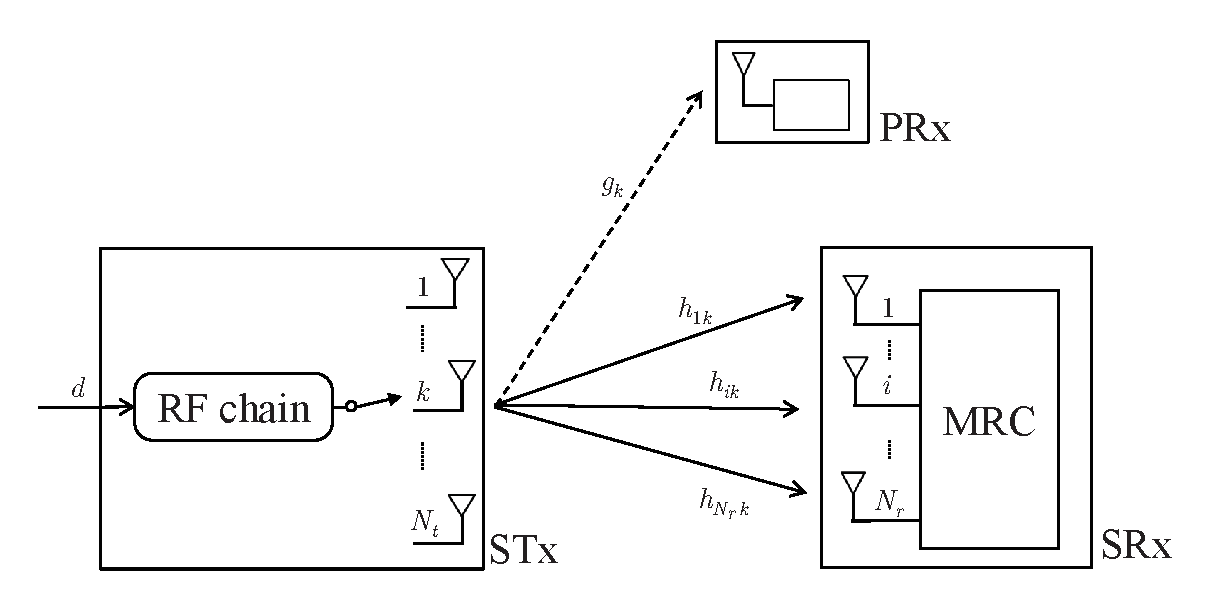
\includegraphics[width=\linewidth]{./model_pdf.eps}
\caption{System model that consists of an STx with $\Nt$ transmit antennas and one RF chain. It transmits data to an SRx with $\Nr$ antennas and causes interference to the PRx.}
\label{fig:MODEL}
\end{figure}



\subsection{Antenna Selection Options and Data Transmission}\label{sec:antenna_selection_options}
The STx transmits with power $\Pt$ a data symbol $\datasymbol$, which is drawn with equal probability from a constellation consisting of $M$ symbols, where $\Pt$ is a system parameter. It can select one out of $\Nt$ antennas or it can also decide to transmit with zero power in order to not interfere with the PRx. For ease of exposition, we denote the latter option as transmitting from a virtual antenna $\nx$, and define $\hk{1\nx} = 0,\ldots,\hk{\Nr\nx} = 0$, and $\gk{\nx}= 0$. 

Let $s\in\allopts$ denote the antenna selected by the STx. At the $\ith$ receive antenna of the SRx, let $\Rsrx$ denote the signal received and let $\Isrx$ denote the interference from PU transmissions. Let the interference at the PRx due to SU transmissions be $\Iprx$. Then, $\Rsrx$ and $\Iprx$ are given by
%
\begin{align}
\label{eq:r_su}
 \Rsrx &= \sqrt{\Pt}\sqrt{\hk{is}} e^{j\thetahk} \datasymbol + \noise + \Isrx, \\
 \label{eq:i}
 \Iprx &= \sqrt{\Pt}\sqrt{\gk{s}} e^{j\thetagk} \datasymbol,
\end{align}
%
where $\expect{|\datasymbol|^2}=1$, $\thetahk$ and $\thetagk$ are the phases of the complex baseband STx-SRx and STx-PRx channel gains, respectively, and $\noise$ is a circular symmetric complex additive white Gaussian RV. We assume $\Isrx$ to be Gaussian. Therefore, $\noise + \Isrx\sim \CN\left(\noisevar\right)$. This is widely assumed in the literature to ensure tractability~\cite{Sarvendranath_2013_TCOM,Wang_2011_TCom, Kashyap_2014_TCOM,Sarvendranath_2014_TCOM}. For example, without it, the maximum likelihood receiver need not reduce to MRC. It is valid even with one primary transmitter (PTx) if the PTx uses a constant amplitude signal to communicate with the PRx~\cite{Kashyap_2014_TCOM}. With multiple PTxs, it is justified by the central limit theorem. This is also valid when the interference seen at the SRx is negligible, which  occurs when the SRx and PTx are far apart~\cite{musavian_2009_tcom,RZhang_2009_TWC,li_2011_pimrc}. We refer the reader to~\cite{das_2015_twc} for an in-depth comparison of this model with other models. 

\subsection{CSI Assumptions and Justifications}
\label{sec:CSI_assumption}  
Before we state the optimal TAS rule problem, we discuss the  CSI assumptions below. 
\begin{enumerate}
\item We assume that the STx knows the STx-SRx channel power gains $\Hmx$, which is possible by exploiting reciprocity~\cite{Hanif_2015_globecom,Sarvendranath_2013_TCOM,Wang_2010_TWC,RZhang_2009_TWC,Sarvendranath_2014_TCOM}. However, it need not know the phase  of any of these channels. The SRx uses a coherent demodulator. Hence, it only needs to know the complex channel gains from the selected antenna of the STx to itself, \ie, $\hk{is}$ and $\thetahk$, for $i\in\nropts$. Inserting a pilot symbol along with the data transmitted by the STx can enable this.  

\item We also assume that the STx knows the STx-PRx channel power gains $\g$, as has been widely assumed in the underlay CR literature~\cite{Hanif_2015_globecom,Sarvendranath_2013_TCOM,Sarvendranath_2014_TCOM,Kong_2011_JCN,Wang_2010_TWC,RZhang_2009_TWC}. 
Different techniques have been studied to obtain  $\g$, which are summarized in~\cite{Zhang_2017_tcom}. These include making the STx sense the primary signal periodically~\cite{Zhao_2008_TSP} or using a power-feedback loop technique~\cite{RZhang_2008_DSAN}. As we shall see, LWIIR  requires the STx to only know if the STx-PRx channel power gain of each antenna exceeds a threshold.  

\end{enumerate}

\subsection{Problem Statement}
\label{sec:problem_statement}
We now formally state our problem. Let $\SEP(\hs)$ denote the instantaneous SEP when antenna $s$ is used for transmission, where $\hs\define\left[\hk{1s},\ldots,\hk{\Nr s} \right]$. From~\cite[eq. (14)]{Chung_2001_TCom}, it is given by  
\begin{equation}
\SEP(\hs) \approx \cone \exp\left({-\frac{\Pt\sumnr\hk{is}}{\ctwo\noisevar} }\right), \,\,\text{for} \,\, 0\leq s \leq \Nt,
\label{eq:isep}
\end{equation} 
where $\cone$ and $\ctwo$ are modulation-specific constants. The summation term $\sumnr\hk{is}$ in~\eqref{eq:isep} arises because the SRx employs MRC. This formula is exact for differential binary phase-shift-keying  with $(\cone,\ctwo) = (0.5,1)$  and non-coherent binary frequency-shift-keying  with  $(\cone,\ctwo) = (0.5,2)$~\cite{Fakhan_2014_TSP}. It is a tight approximation for many constellations, e.g.,  $(\cone,\ctwo)=(0.5,1.7)$ for QPSK,  $(\cone,\ctwo)=(0.6,5.5)$ for 8-PSK, and  $(\cone,\ctwo )=(0.8,8.2)$ for 16-QAM. 


{\em Comments:}
\begin{itemize}

\item Even with zero transmit power ($s=\nx$), it follows from~\eqref{eq:isep} that the SEP is\footnote{For a constellation of size $M$, the SEP with zero transmit power is exactly $\zerosep\define 1-\left(1/M\right)$. While we design the TAS rule using~\eqref{eq:isep} for all $\Nt+1$ options in order to ensure tractability, we shall use $\SEP(\h_0) = \zerosep$ in the analysis in Section~\ref{sec:SEPanalysis} in order to ensure its accuracy.} $\cone<1$. From~\eqref{eq:isep}, the SEP will be strictly less than $\cone$ when one of the $1,\ldots,\Nt$ antennas is selected and a  transmit power $\Pt$ is used. Therefore, $\cone$ can be interpreted to be a worst-case penalty associated with using the zero transmit power option. It ensures that the optimal TAS rule does not always select the trivial $s=\nx$ option to satisfy the interference constraint~\cite{Kashyap_2014_TCOM,Sarvendranath_2013_TCOM}. 	


\item Our model is based on binary power control, which has been studied widely~\cite{Kashyap_2013_TWC,Kashyap_2014_TCOM,Hanif_2015_globecom,Sarvendranath_2013_TCOM} and requires analytical methods that are different from those used for continuous power control~\cite{Sarvendranath_2014_TCOM}. It is practically relevant because it enables the use of more energy-efficient power amplifiers.


\end{itemize}


{\em TAS Rule Definition:} A TAS rule $\asrule:\brac{\mathbb{R}^{+}}^{\Nr}\times\brac{\mathbb{R}^{+}}^{\Nt} \times \brac{\mathbb{R}^{+}}^{\Nt} \rightarrow \allopts$ is a mapping from $\left(\Hmx,\g\right)$ to the set of $\Nt+1$ available transmit antennas. Thus, $s = \phi(\Hmx,\g)$.

{\em Interference-Outage Constraint:}
From~\eqref{eq:i}, the instantaneous interference power at the PRx is $\Pt\gk{s}$. Therefore, the probability that it exceeds an interference power threshold $\itau$ is equal to $\prob{\Pt\gk{s}>\itau}$. It depends on the TAS rule used through $s$. From the perspective of the PRx,  $\Hmx$ and $\g$ are random, and so is $s$. Then, from its perspective,  the interference-outage constraint can be specified as  the following probabilistic constraint: 
\begin{equation}
\prob{\Pt\gk{s}>\itau} \leq \outmax,
\label{eq:iop_cons}
\end{equation}
where $\outmax$ is the maximum allowed interference-outage probability. We note that this constraint becomes deterministic for the STx when it knows the STx-PRx channel power gains. 


Let $\asspan$ be the set of all TAS rules. Our goal is to find the optimal TAS rule $\phi^{*}\in\asspan$ that minimizes the average SEP of the secondary system subject to the interference-outage constraint. It can be mathematically stated as the  following stochastic, constrained optimization problem $\optproblem$:
\begin{align}
\label{eq:objective}
\optproblem: \quad \min_{\asrule\,\in\,\asspan} \quad
&\explow{\Hmx,\g}{\SEP(\hs)} \\
\label{eq:cons}
\text{s.t.} \quad &\prob{\Pt\gk{s}>\itau} \leq \outmax, \\
 &s = \phi(\Hmx,\g). 
\end{align}
%
\begin{center}
	\begin{table}
		\caption{Key notations}
		\label{tab:notations}
		\centering
		\begin{tabular}{l l l}
			\hline
			$\Hmx=[\hk{ik}]$                 & STx-SRx channel power gain matrix    \\ \hline
			$\g = [\gk{1},\ldots,\gk{\Nt}] $ & STx-PRx channel power gain vector    \\ \hline
			$\Nt$     		                 & Number of transmit antennas at the STx     \\ \hline
			$\Nr$            		         & Number of receive antennas at the SRx    \\ \hline
			$\Pt$, $\snr$                    & Fixed transmit power and SNR             \\ \hline
			$\itau$               & Interference power threshold     \\ \hline
			$\outmax$               &  Maximum interference-outage allowed    \\ \hline
			$s$                              & Index of the antenna selected      \\ \hline
			$\cone$, $\ctwo$                 & Modulation parameters         \\ \hline
			$\lam$                    & Interference-outage penalty factor  \\ \hline
			$\un$                    & Unconstrained interference-outage probability \\ \hline
		\end{tabular}
	\end{table}
\end{center}
%

\section{LWIIR, Its Interference-Outage analysis, and optimality}
\label{sec:analysis}
%
We now propose LWIIR, and characterize its properties and its interference-outage probability. Using these, we prove that LWIIR solves  $\optproblem$ for the general class of continuous fading models. 


\subsection{LWIIR and Its Properties}
\label{sec:lambda_rule}
Let 
\begin{equation}
\yk{k} \define \frac{\SEP(\bhk{k})}{\cone} = \exp\left({- \frac{\Pt\sum_{i=1}^{\Nr}\hk{ik}}{\ctwo\noisevar} }\right),  
\label{eq:yi_def}
\end{equation}
for  $0\leq k \leq\Nt$. LWIIR is defined in terms of a parameter $\lam \in \left[0, \cone\right]$, and is denoted by $\callamrule$. It is as follows:
\begin{equation}
\callamrule: \quad s=\argmin\limits_{k\in\allopts} \left\{ \ykplusgk{k} \right\}.
\label{eq:lam_weight_rule}
\end{equation}

To understand the behavior of $\callamrule$, we first introduce the following terminology. We shall refer to $\ykplusgkinl{k}$ as the {\em selection metric} of antenna $k$, for $0\leq k \leq\Nt$. Thus, LWIIR selects the antenna with the smallest selection metric. Further, we shall call an antenna $k$ for which $\gklttaubyptinl{k} $ as an {\em outage-compatible} antenna. Otherwise, we shall call it an {\em outage-incompatible} antenna.  Clearly, antenna zero is always outage-compatible, and its selection metric is $\yk{0}=1$, which is independent of the modulation used. We shall refer to $\lam$ as the {\em interference-outage penalty factor} as it increases the selection metric of, i.e., it penalizes, an outage-incompatible antenna. Note that given $\Hmx$ and $\g$, LWIIR is a deterministic rule for STx.


{\em Behavior of LWIIR for Different $\lam$ Values:}
\begin{enumerate}
\item For $\lam=0$, the selection metric of antenna $k$ is $\yk{k}$. As $\sumnr\hk{ik}\geq 0$, it follows from~\eqref{eq:yi_def} that $\yk{0}=1\geq\yk{1},\ldots,\yk{0}\geq\yk{\Nt}$. And,   $\yk{1},\ldots,\yk{\Nt}$ are monotonically decreasing functions of $\sumnr\hk{i1},\ldots,\sumnr\hk{i\Nt}$, respectively. Hence, antenna $\nx$ will not be selected. Therefore, 
\begin{equation}
\caluncons: s = \argmin\limits_{k\in\antopts} \left\{ \yk{k} \right\} = \argmax\limits_{k\in\antopts} \left\{\sumnr \hk{ik} \right\}.
\label{eq:uncons_simple}
\end{equation}
%
From~\eqref{eq:isep}, $\caluncons$ is clearly the optimal  rule if the interference-outage constraint in~\eqref{eq:cons} is inactive. We shall, therefore, refer to $\caluncons$ as the {\em interference unconstrained} rule henceforth. Its interference-outage probability $\un$ is given by
%
\begin{equation}
\un= \prob{\gkgrtaubypt{s}}= F^c_{\gk{1}}\left({\taubypt}\right).
\label{eq:uncomsoutage}
\end{equation}
%
The second equality above follows because the antenna $s$ selected by $\caluncons$ does not depend on $\g$, and $\gk{1},\ldots,\gk{\Nt}$ are i.i.d. Thus, $\caluncons$ is the optimal  rule when $\outmax \geq \un$. 

\item For $0<\lam<\cone$, the selection metric of antenna $k$ is a linear combination of  an exponentially decreasing function of $\sumnr\hk{ik}$ and $\indic{\gkgrtaubyptinl{k}}$, which is a discontinuous function of $\gk{k}$. A three-dimensional view of this selection metric as a function of $\sumnr\hk{ik}$ and $\gk{k}$ is shown in Figure~\ref{fig:metric}. Notice its discontinuous behavior, which happens at $\gk{k}= \itau/\Pt$ and is different from the TAS rules in~\cite{Hanif_2015_globecom,Sarvendranath_2013_TCOM,Sarvendranath_2014_TCOM,Wang_2011_TCom,Fakhan_2014_TSP}.

\item For $\lam=\cone$, the selection metric of any outage-incompatible antenna $k$ is  $\yk{k}+1> \yk{0}$. Therefore, LWIIR will select an antenna $k$ with the largest $\sumnr\hk{ik}$ only from the set of outage-compatible antennas. For this special case, it is equivalent to the HYA rule, which was proposed for the  peak interference constraint.



\end{enumerate}
\begin{figure}
	\centering 
	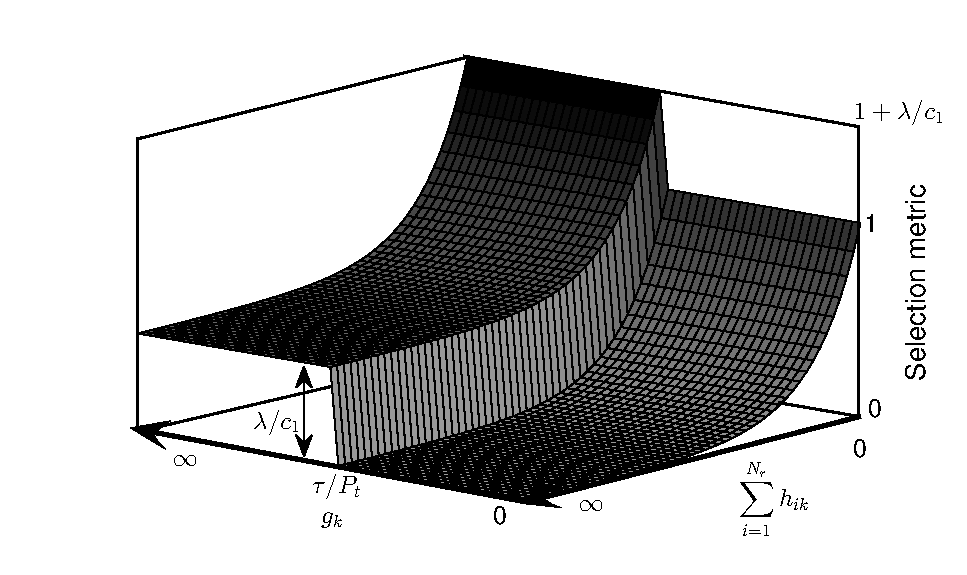
\includegraphics[width=\linewidth]{./selection_metric_3d.eps}
	\caption{Selection metric of antenna $k$ as a function of $\sumnr\hk{ik}$ and $\gk{k}$.}
	\label{fig:metric}
\end{figure}

\subsection{Interference-Outage Probability and Optimality of LWIIR} 
\label{sec:out_prob_opt}
We first derive the interference-outage probability of LWIIR in terms of the probability distribution of $\yk{1},\ldots,\yk{\Nt}$. Since $\yk{1},\ldots,\yk{\Nt}$ are identically distributed, we denote their marginal CCDF and PDF by $F_{y}^{c}(\cdot)$ and $f_{y}(\cdot)$, respectively. 
\begin{lemma}
\label{lem:outage_Nt}
The interference-outage probability $\outlam$ of LWIIR, for $0\leq\lam\leq\cone$, is given by
\begin{equation}
\label{eq:pr_outage_ccdf} 
\outlam\!  =\!  \Nt\un\!\!\! \int_{0}^{1-\lambycone}\!\!	
\left[\un\!F_{y}^{c}\!\left(x\right) \!+\! \left(1 \!-\!\un\right)\!F_{y}^{c}\!\left(x\!+\!\lambycone\right)\! \right]^{\!\Nt-1}\!\!\!\! f_{y}(x)dx.
\end{equation}
For the class of continuous fading models, $\outlam$ is a continuous and strictly monotonically decreasing function of $\lam$. Furthermore, for any $\outmax\in[0,\un]$, a unique $\lam\in[0,\cone]$ exists such that $\outlam=\outmax$. 
\end{lemma}
%
\begin{IEEEproof}
The proof is given in Appendix~\ref{proof:outage_Nt}.
\end{IEEEproof}
%

Using Lemma~\ref{lem:outage_Nt}, we prove the following result. 
%
\begin{result}
\label{res:selection_rule_on_off}
The optimal TAS rule that solves $\optproblem$ lies in the set of rules $\set{\callamrule:0\leq\lam\leq\cone}$. If $\outmax\geq\un$, then it is given by $\caluncons$. Else, for $0\leq\outmax<\un$, it is given by $\callamstarrule$, where $\lamstar>0$  is the solution of $\outlam=\outmax$. Such a choice of $\lamstar$ is unique, strictly positive, and always exists. 
\end{result}
%                
\begin{IEEEproof}
   The proof is given in Appendix~\ref{proof:selection_rule_on_off}.
\end{IEEEproof}
%

This result brings out how the interference constraint fundamentally affects the structure of the optimal TAS rule. We obtain $\lamstar$ by equating $\outlam$ in~\eqref{eq:pr_outage_ccdf} to $\outmax$ and solving it numerically, for example, using the bisection method. The following approach circumvents this problem.  

Replacing $x+\left( \lambyconeinl\right) $ with $\lambyconeinl$ in~\eqref{eq:pr_outage_ccdf} yields the following closed-form bound for $\outlam$: 
%
\begin{multline}
\label{eq:pr_outage_ub}
\outlam  \leq \left[ \un + \left(1-\un\right)F_{y}^{c}\left(\lambycone\right)  \right]^{\Nt} \\ -  \left[ \un F_{y}^{c}\left(1-\lambycone\right) + \left(1-\un\right)F_{y}^{c}\left(\lambycone\right)  \right]^{\Nt}.
\end{multline}



%
For $\Nt = 2$, the following different, simpler bound can also be derived: 
%
\begin{equation}
\label{eq:two_Nt_UB}
\outlam \leq \un^2 + 2\un(1-\un)F_{y}^{c}\left(\lambycone\right),
\end{equation}
which shows that $\outlam$ is an increasing function of $\cone$ since $F_{y}^{c}(\cdot)$ is a monotonically decreasing function. For example, for Rayleigh fading and $\Nr=1$, equating~\eqref{eq:two_Nt_UB} to $\outmax$ yields the following closed-form upper bound for $\lam$ that holds for $\itau\geq-\left( \Pt\mug/{2}\right) \ln\left({\outmax}\right)$:
%
\begin{equation}
\label{eq:two_Nt_lam}
\lam \leq \cone \left( \frac{2\un - \un^2 - \outmax}{2\un(1-\un)} \right)^{\snrbyal[]}.
\end{equation} 




\subsection{Insights: A Simpler, Intuitive  TAS Rule and Its Interference-Outage Probability}\label{sec:insights}

In this section, we gain new insights about LWIIR when $\lam \tendsto \cone$. Intuitively, this occurs when the interference-outage constraint is very tight.



For a given realization of the channel gains, let $\goodset$ denote the set of all outage-compatible antennas among the antennas $1,2,\ldots,\Nt$. Now consider the following two cases: (i)~{\em $\goodset\neq~\nullset$:} From Comment 3 in Section~\ref{sec:lambda_rule}, it follows that as $\lam \tendsto \cone$, $\callamrule$ becomes 
%
\begin{equation}
\label{eq:hp_rule_G_not_empty}
s = \argmax_{k\in\goodset}\left\lbrace \sumnr \hk{ik}\right\rbrace. 
\end{equation}
%
(ii)~{\em $\goodset= \nullset$:} Here, $\callamrule$ selects the antenna $s = \argmin\left\lbrace  \yk{0},\yk{1}+\lambyconeinl,\ldots,\yk{\Nt}+\lambyconeinl \right\rbrace$. Using $\yk{0}=1$ and \eqref{eq:yi_def}, the selection rule for this case simplifies  to  
\begin{equation}
\label{eq:hp_rule_G_empty}
s = \!\left\{\!\!
\begin{array}{ll}
0,  \hspace{50pt}\text{if}~\sumnr\!\hk{i1}\!\!\!&	\!\!\leq \gammath,\ldots, \sumnr\hk{i\Nt}\leq\gammath, \\ 
\argmax\limits_{k\in\antopts}\!\!\left\lbrace \!\sumnr\hk{ik}\!\right\rbrace,\!\! &\text{otherwise},
\end{array}\right.
\end{equation}
where $\gammath\define\igammainline$. Hence, $\callamrule$ selects antenna $s\neq0$ if and only if there is at least one antenna $k\in\antopts$ for which $\sumnr \hk{ik}$ exceeds $\gammath$. Else, $s=0$. 


{\em Interference-Outage Probability:} For the above selection rule, it can be shown that
\begin{equation}
\label{eq:pr_outage_hp}
\outlam = \un^{\Nt} - \un^{\Nt}\left(\ccdfyrv{1-\lambycone} \right)^{\Nt}.
\end{equation}
%
From~\eqref{eq:pr_outage_hp}, we see that as $\lam\tendsto\cone$, $\outlam$ decreases as $\un$ decreases or as $\Nt$ increases. 
For Rayleigh fading and $\Nr=1$, equating~\eqref{eq:pr_outage_hp} with $\outmax$ yields the following closed-form expression for $\lam$ for $\itau<-\left({\Pt\mug}/{\Nt}\right) \ln\left({\outmax}\right)$: 
\begin{equation}
\label{eq:lam_asym}
\lam  =  \cone - \cone\left(1 - \left[1 - \frac{\outmax}{\un^{\Nt}}\right]^{\frac{1}{\Nt}} \right)^{\snrbyal[]}.
\end{equation}
%
Form~\eqref{eq:two_Nt_lam} and~\eqref{eq:lam_asym} we see that $\lam$ increases as $\cone$ increases and  decreases as $\outmax$ increases.



\section{SEP Analysis of LWIIR}
\label{sec:SEPanalysis}
We derive a general expression for the average SEP of LWIIR, which we denote by  $\avgSEP$. It holds for any number of transmit and receive antennas. 

\begin{result}
\label{thm:SEP_exact_Nt_gen}
$\avgSEP$ of $\callamrule$ is given by
\begin{equation}
\label{eq:SEP_Nt_gen} 
\avgSEP= \zerosep\left[\unccdfygen{\un}{1-\lambycone}\right]^{\Nt} + \termtwo,
\end{equation}
%
where $\zerosep = 1 - \left( {1}/{M}\right) $ and
\begin{align}
\termtwo = &\Nt\cone(1-\un)\int_{0}^{\lambycone} \left[\un + \unccdfygen{(1-\un)}{x}\right]^{\Nt-1} x\pdfyNrgen{x} dx\nonumber\\
&+ \Nt\cone \int_{0}^{1-\lambycone}\!\!
\left[\unccdfygen{\un}{x} +\unccdfygen{(1-\un)}{x+\lambycone}  \right]^{\Nt-1}\nonumber\\
&\times\left(\un x\pdfyNrgen{x} + (1-\un)\left(x + \lambycone\right) \pdfyNrgen{x + \lambycone}\right) dx.
\label{eq:termtwo_gen}
\end{align}
%
\end{result}
%
\begin{IEEEproof}
The proof is given in Appendix~\ref{proof:SEP_exact_Nt_gen}.
\end{IEEEproof}
%


{\em Example:} For Rayleigh fading, in which $\hk{ik}$ and $\gk{k}$ are i.i.d.\ exponential RVs with means $\muh$ and $\mug$, respectively, it can be shown that $\un=\inlccdfg[]$. Let $\snr\define\Pt\muh/\noisevar$ denote the mean signal-to-noise-ratio (SNR) of the SU. Thus, the CCDF and PDF of the RV $\yk{1}$ are given by 
\begin{align}
\label{eq:ccdfyNr}
\ccdfyrv{x} &= 1 - x^{\albysnr} \sum_{m=0}^{\Nr-1} \frac{\left(-\albysnr \ln(x) \right)^{m}}{m!}, \,\, \text{for}\,\, x \in (0,1],\\
\label{eq:pdfyNr}
\pdfyNrgen{x} &= \pdfyNr, \, \text{for}\,  x \in (0,1].
\end{align}
\newcommand{\tl}{t_l}

Note that further simplification of~\eqref{eq:termtwo_gen} to an integral-free form is not possible because of the involved form of its two integrands.  However, it can be approximated to the following integral-free summation:
%
\begin{align}
\label{eq:termtwo_approx}
\termtwo \approx &\Nt\lam(1-\un) \!\sum_{\lidx=1}^{n}  w_{\lidx}\!\left[\un + \unccdfygen{(1-\un)}{t_l}\!\right]^{\Nt-1} t_l f_{y}\left(t_l\right) \nonumber\\
&+ \Nt\left( \cone - \lam \right) \sum_{\lidx=1}^{n} w_{\lidx}
\left[\unccdfygen{\un}{\vl} +\unccdfygen{(1-\un)}{\xl}  \right]^{\Nt-1} \nonumber\\
&\times\left(\un \vl \pdfyNrgen{\vl} + (1-\un) \xl \pdfyNrgen{ \xl }\right),
\end{align}
where  $t_l={\lambda z_{l}}/{c_1}$, $\vl\define\left(1-\left( \lambyconeinl\right) \right) z_{\lidx}$,  $\xl=\vl+\left( \lambyconeinl\right) $, $\gqsym$ and $\gqwt$ are the $n$ abscissas and weights, respectively, for Gaussian integration of moments~\cite[pp. 921--922]{abramowitz_stegun}.


\subsection{Insights: Rayleigh Fading and $\Nr=1$}
\label{sec:spec_case_Nr_1} 
For this case,~\eqref{eq:ccdfyNr} and~\eqref{eq:pdfyNr} simplify to $F_{y}^{c}(x) = 1-x^{\albysnr}$ and $f_{y}(x) = \al x^{\albysnr-1}/\snr$, for $x \in (0,1]$. Upon substituting these in~\eqref{eq:SEP_Nt_gen}, $\avgSEP$ simplifies to 
%
\begin{align}
\label{eq:avgSEPoneNr} 
\avgSEP =&\zerosep\,\un^{\Nt}\left[1-\left(1-\lambycone\right)^{\albysnr[]}\right]^{\Nt} \nonumber\\
&+ \frac{\Nt\un^{\Nt}\al\lam}{\snr} \sum_{k=0}^{\Nt-1}\sum_{\lidx=0}^{k} \frac{\nck{\Nt-1}{k} \nck{k}{\lidx}\left( \lambycone\right) ^{\albysnr[(\lidx+1)]} }{(-1)^{\lidx} \left( \albysnr[(\lidx+1)]+1\right) }\nonumber\\ 
&\times\frac{\left(1-\un\right)^{k+1}}{\un^{k+1}}  + \frac{\Nt\cone\al}{\snr} \sum_{k=0}^{\Nt-1} \sum_{\lidx=0}^{k} \sum_{\midx=0}^{\Nt-k-1}  \!\!\!\binom{\Nt-1}{k}\nonumber \\ 
&\times\binom{k}{\lidx} \binom{\Nt-k-1}{\midx}(-1)^{\lidx+\midx} \un^{k} (1-\un)^{\Nt-k-1} \nonumber \\
&\times\left[ \un\psifun{\midx}{\lidx+1} +  \left(1-\un\right) \psifun{\midx+1}{\lidx} \right]
,
\end{align}
where $\psifun{k_1}{k_2} = \int_{0}^{1-\lambycone} \left(x+\left( \lambyconeinl\right) \right)^{\albysnrinl[k_1]} x^{\albysnrinl[k_2]} \,dx$. In general, $\psifun{k_1}{k_2}$ can be computed accurately as a sum of $n$  terms using Gaussian integration of moments as follows: 
\begin{equation}
\psifun{k_1}{k_2}  = {\onemlc} \sum_{\lidx=1}^{n} \gqwt {\left(\vl +\lambycone\right)}^{\albysnr[k_1]} \vl^{\albysnr[k_2]} + \error.
\label{eq:gauss_quad}
\end{equation}
The error term $\error$ decreases as $O(1/n^2)$~\cite{Xiang_2012_SIAM}, where $O(\cdot)$ is as per the Bachmann-Landau notation~\cite[Chap. 3]{CLRS_algo_book}. In Section~\ref{sec:results}, we will see that~\eqref{eq:gauss_quad}  is accurate even for $n$ as small as 4. Furthermore, for $\lam\in({\cone}/{2}, \cone]$, $\psifun{k_1}{k_2}$ can be written as an infinite series~\cite{gradshteyn00_book}:
%
\begin{equation}
\psifun{k_1}{k_2} = \sum_{\midx=0}^{\infty} \frac{\Gamma\left(\akone+1 \right) \left( \lambycone\right) ^{\albysnr[k_1]  - \midx} \left(1-\lambycone\right)^{\albysnr[k_2]+\midx+1}}{\Gamma\left(\akone-\midx+1 \right)\midx! \left(\albysnr[k_2]+\midx+1\right)}. 
\label{eq:inf_sum}
\end{equation}
Four terms in the above summation turn out to be sufficient. 
 
{\em Insights From~\eqref{eq:avgSEPoneNr}:} The first term corresponds to the average SEP due to $s=\nx$. It increases as $\lam$ increases. This is because a higher $\lam$ corresponds to a tighter interference-outage constraint, which increases the probability of selecting $s=\nx$. It is also an exponentially decreasing function of $\itau$ and $\Nt$. The second and third terms correspond to the average SEP due to the transmissions with power $\Pt$. The second term is directly proportional to $\lam$ and is inversely proportional to $\cone$.
%



\section{Impact of Imperfect CSI on LWIIR}
\label{sec:imperfectcsi}
We now study the behavior of LWIIR when the STx has imperfect estimates of the STx-SRx and STx-PRx channel power gains, as is the case in practice, for Rayleigh fading. For tractability, we assume that the secondary receiver SRx knows perfectly the $\Nr$ complex channel gains for the transmit antenna selected.  


{\em Channel Estimation Model}: We consider the minimum mean square error (MMSE) channel estimation model~\cite{Sboui_2013_TWC,Kashyap_2014_TCOM,musavian_2009_tcom,Zhang_2017_tcom,Kashyap_2015_wicomlet}. For the $\kth$ transmit antenna of the STx, let $ \sugain{ik}= \sqrt{\hk{ik}}e^{j\suchph_{ik}}\sim\CN\left(\muh\right)$ denote the baseband channel gain from it  to the $\ith$ receive antenna of the SRx, and let $\pugain{k} = \sqrt{\gk{k}}e^{j\puchph_{k}}\sim\CN\left(\mug\right)$ denote the baseband channel gain from it to the PRx. Let $\sugainhat{ik}$ and $\pugainhat{k}$ denote the MMSE estimates of $\sugain{ik}$ and $\pugain{k}$, respectively. These can be obtained from pilot transmissions by the SRx and PRx with powers $\hpilotpower$ and $\gpilotpower$, respectively.  It can be shown that  $\sugainhat{ik}\sim\CN\left(\muhhat \right)$ and $\pugainhat{k}\sim \CN\left(\mughat\right)$, where  $\muhhat ={\hpilotpower\mu^2_{\such}}/{\left( \hpilotpower\muh+1\right)}$ and $\mughat = {\gpilotpower\mu^2_{\puch}}/{\left( \gpilotpower\mug+1\right)}$~\cite{Kashyap_2014_TCOM}.  
This implies that the channel power gain estimates $\hkhat{ik}=|\sugainhat{ik}|^2$ and $\gkhat{k}=|\pugainhat{k}|^2$ are i.i.d. exponential RVs with means $\muhhat$ and $\mughat$, respectively. Furthermore, the correlation coefficient  of  $\hk{ik}$ and $\hkhat{ik}$ is $\rhoh\define{\hpilotpower\muh}/{\left( \hpilotpower\muh + 1\right) }$, and that of $\gk{k}$ and $\gkhat{k}$ is $\rhog \define{\gpilotpower\mug}/{\left( \gpilotpower\mug + 1\right) }$. 

The STx selects its transmit antenna on the basis of the imperfect estimates of $\Hmx$ and $\g$ as follows:  
\begin{equation}
\callamrule:\quad s=\argmin\limits_{k\in\allopts} \left\{ \ykhatplusgkhat{k} \right\},
\label{eq:shat}
\end{equation}
%
where 
\begin{equation}
\ykhat{k} \define  \exp\left({- \frac{\Pt\sum_{i=1}^{\Nr}\hkhat{ik}}{\ctwo\noisevar} }\right), \quad \text{for} \quad 0\leq k \leq\Nt,
\label{eq:yihat_def}
\end{equation}
$\hkhat{1\nx} \define 0,\ldots,\hkhat{\Nr\nx} \define 0$, and $\gkhat{\nx} \define 0$. Let $F_{\yhat}^{c}(\cdot)$ and $f_{\yhat}(\cdot)$ denote the CCDF and PDF, respectively, of the i.i.d. RVs $\ykhat{1},\dots,\ykhat{\Nt}$. They are given by
%
\begin{align}
\label{eq:CCCDF_yhat}
\ccdfyrv{x} &= 1 - x^{\albysnrhat} \sum_{m=0}^{\Nr-1} \frac{\left(-\albysnrhat \ln(x) \right)^{m}}{m!}, \,\, \text{for}\,\, x \in (0,1],\\
\label{eq:pdfyNrhat}
\pdfyNrgen{x} &= \frac{\left(\albysnrhat\right)^{\Nr}\left(-\ln\left({x}\right)\right)^{\Nr-1}x^{\albysnrhat[]-1}}{(\Nr-1)!}, \,\, \text{for}\,\,  x \in (0,1].
\end{align}
Let 
\begin{equation}
\unhat\define\ccdfghat\, \text{and}\,\,\, \snrhat\define\frac{\Pt\muhhat}{\noisevar}.  
\end{equation}


\subsubsection{Average SEP} 
The average SEP of the TAS rule in~\eqref{eq:shat} is given as follows. 
\begin{result}
\label{thm:avg_SEP_imperfect}
$\avgSEP$ of $\callamrule$ for an $\Nt\times\Nr$ CR system with imperfect CSI at the STx is given by
\begin{align}
\label{eq:avg_SEP_imperfect}
\avgSEP =& \zerosep\left[\unccdfyhat{\unhat}{1-\lambycone}\right]^{\Nt}
+\frac{\Nt \T^{\Nr}\cone(1-\unhat)}{(\Nr-1)!}\nonumber\\
&\times \int_{0}^{\lambycone} \!\!\left[\unhat + \unccdfyhat{(1-\unhat)}{x}\right]^{\Nt-1}\!\! \yhattimespdfyNr dx\nonumber\\
& + \frac{\Nt \T^{\Nr}\cone}{(\Nr-1)!} \int_{0}^{1-\lambycone}
\left(  \unhat\yhattimespdfyNr
 \right. \nonumber \\
& + \left. (1-\unhat)\yhatpluslamtimespdfyNr \right) \nonumber \\
& \times \left[\unccdfyhat{\unhat}{x} + \unccdfyhat{(1-\unhat)}{x+\lambycone} \right]^{\Nt-1} dx,
\end{align}
where $\T \define \Tc$ and $\D \define \Dc$.    
\end{result}
\begin{IEEEproof}
	The proof is given in Appendix~\ref{proof:avg_SEP_imperfect_CSI}.
\end{IEEEproof}


Further simplification of $\avgSEP$ in~\eqref{eq:avg_SEP_imperfect} is not possible due to the involved form of the integrand. However, for $\Nr=1$, simplified expressions similar to~\eqref{eq:avgSEPoneNr} can be obtained. 



\subsubsection{Interference-Outage Probability} 
%
\begin{result}
\label{thm:outage_imperfect_CSI}
  The interference-outage probability $\outlam$ of $\callamrule$ with imperfect CSI is given by
\begin{align}
\label{eq:pr_outage_impefect} 
\!\outlam \!=& \Nt \!\int_{0}^{1-\lambycone} 	
\!\left[ \unhat F_{\yhat}^{c}\left(x\right) + \left(1 -\unhat\right)F_{\yhat}^{c}\left(x+\lambycone\right)\right]^{\Nt-1}\nonumber\\
&\times \left( (\un - \Probglt) f_{\yhat}\left(x\right)  +  \Probglt f_{\yhat}\left( x+\lambycone\right) \right) dx\nonumber\\
&+ \frac{ \Probglt}{1 - \unhat} \left( 1 - \left[\unhat + \left(1 -\unhat\right)F_{\yhat}^{c}\left(\lambycone\right)  \right]^{\Nt}  \right),
\end{align}
%
where 
$\Probglt \!=\! \un  Q_1\!\!\left(\!\frac{\gpilotpower}{\rhog } \sqrt{\frac{2\itau}{ \gpilotpower\Pt}},\sqrt{\frac{2 \gpilotpower\itau}{\Pt}}\!\right) \! - \unhat  Q_1\!\left(\!\sqrt{\frac{2\itau \gpilotpower}{\rhog \Pt}},\!\sqrt{\frac{2\itau\gpilotpower}{\rhog \Pt}} \!\right)\!$ and  $Q_1(\cdot,\cdot)$ is the Marcum-Q function~\cite[eq. (4.34)]{simon_alouini_book}. 
\end{result}
%
\begin{IEEEproof}
	The proof is given in Appendix~\ref{proof:outage_imperfect_CSI}.
\end{IEEEproof}
%

In the interference-outage unconstrained case $\left(\lam=0\right)$, $\outlam$ in~\eqref{eq:pr_outage_impefect} reduces to $\un$ even with imperfect CSI. This is because  the selected antenna does not depend on the  STx-PRx channel power gain estimates. In the other extreme case of $\lam = \cone$, which is equivalent to the peak interference constraint, $\outlam$ simplifies to ${\Probglt \left( 1-\unhat^{\Nt}\right)}/( {1-\unhat})>0 $, while it is zero for perfect CSI.  Similar to~\eqref{eq:pr_outage_ub}, 
we can show that $\outlam$ in~\eqref{eq:pr_outage_impefect}  is upper bounded as 
\begin{align}
\outlam  \leq  &\frac{ \Probglt \left( 1-\unhat^{\Nt}\right)}{1-\unhat} + \frac{\un - \Probglt}{\unhat}\!\!\left( \left[\unhat + \left(1-\unhat\right)F_{\yhat}^{c}\left(\lambycone\right)\right]^{\Nt} \right. \nonumber \\ &\left. - \left[ \unhat F_{\yhat}^{c}\left(1-\lambycone\right) + \left(1-\unhat\right)F_{\yhat}^{c}\left(\lambycone\right)\right]^{\Nt}\right).
\end{align}



\section{Numerical Results and Performance Benchmarking}
\label{sec:results}
We now present Monte Carlo simulations that measure the average SEP over $10^6$ data symbols for both perfect and imperfect CSI. These simulate the entire transmit and receive chains and do not assume the formula in~\eqref{eq:isep}; therefore, they independently verify our problem formulation and analysis. We set $\lam$ as  $\lamstar$, which is characterized in Result~\ref{res:selection_rule_on_off}. We set $\noisevar =1$ and $\muh =\mug = 1$, and show results for Rayleigh fading. 

Figure~\ref{fig:SEP_vs_tau} plots the average SEP of LWIIR as a function of the interference power threshold $\itau$. The exact analytical expression in~\eqref{eq:SEP_Nt_gen} and its approximation in~\eqref{eq:termtwo_approx} with $n=4$ terms are shown. They match well with the simulations. The average SEP behavior depends on which of the two following regions $\itau$ lies in. (i) {\em Interference-outage constrained region $(\itau < 8.6$~dB), in which $\lam>0$:} The average SEP decreases as $\itau$ increases because the interference power allowed at the PRx increases; (ii) {\em Interference-outage unconstrained region $(\itau \geq 8.6$~dB), in which $\lam=0$:} The average SEP is a constant as LWIIR reduces to the interference unconstrained rule $\caluncons$. It decreases exponentially as $\Nt$ or $\Nr$ increase.  Also plotted is the average SEP of LWIIR when $\lam$ is obtained by equating the  upper bound for $\outlam$ in~\eqref{eq:pr_outage_ub} to  $\outmax$. We see that the degradation in the average SEP  is negligible when compared to using $\lam^*$. Given its integral-free form,~\eqref{eq:pr_outage_ub} makes it easier to implement LWIIR. 
%
\begin{figure}
  \centering 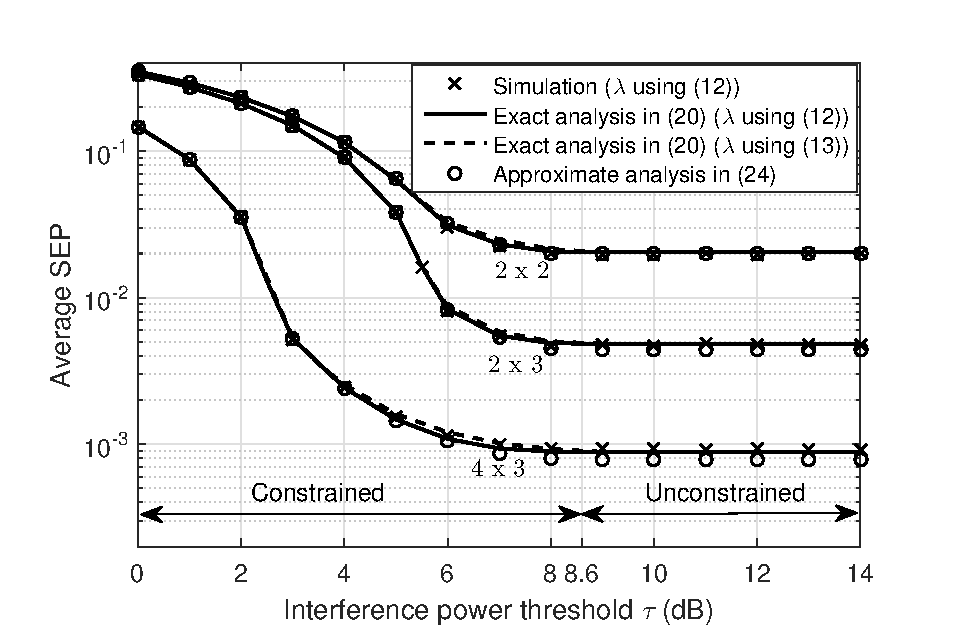
\includegraphics[width=\linewidth]{./PCSI_SEP_vs_tau_pout_10_PT_5dB_Nt_2_4_Nr_2_3_M_4.eps}
  \caption{Average SEP as a function of interference power threshold $\itau$ for different $\Nt \times \Nr$ values ($\outmax=0.1$,  $\Pt = 5$~dB, and QPSK).}
\label{fig:SEP_vs_tau}
\end{figure}

Figure~\ref{fig:SEP_vs_tau_QAM} plots the average SEP as a function of  $\itau$ for different constellations and for two values of $\outmax$. The average SEP formula for $\Nr=1$ in~\eqref{eq:avgSEPoneNr} and its approximation in~\eqref{eq:gauss_quad} with $n=4$ terms for 16-QAM and $n=8$ terms for 8-PSK are also plotted. These match well with the simulations. In the interference-outage constrained region, the average SEP decreases as $\outmax$ increases as the interference constraint becomes more relaxed. In the interference-outage unconstrained region, an error floor that is  independent of $\outmax$ arises.  
%
\begin{figure}
	\centering 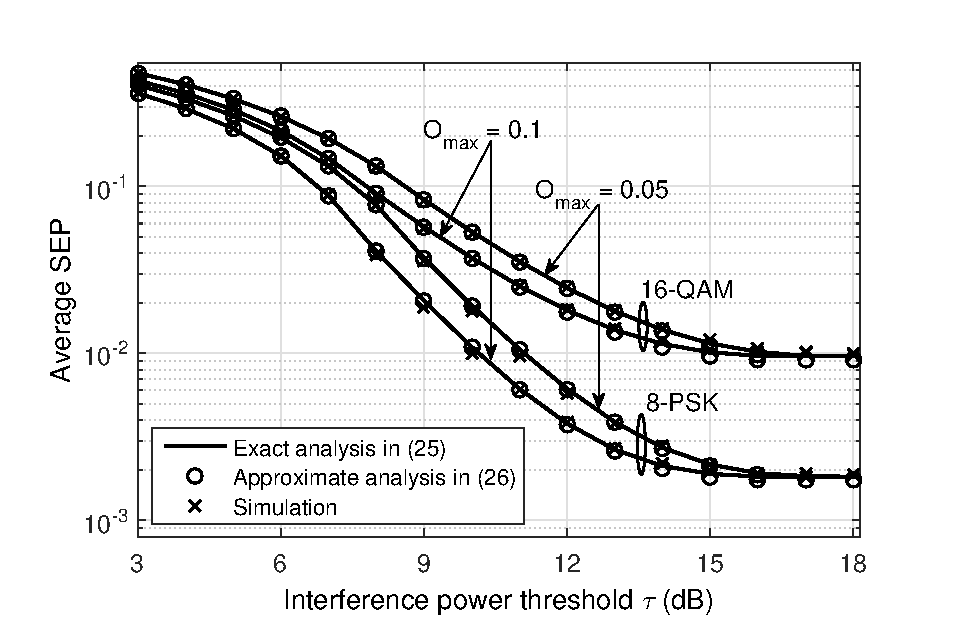
\includegraphics[width=\linewidth]{./CURVE_FIT_SEP_vs_tau_pout_5_10_PT_13dB_Nt_8_M_8_16.eps}
	\caption{Average SEP as a function of $\itau$ for 8-PSK and 16-QAM for different values of $\outmax$ ($\Pt = 13$~dB, $\Nt=8$, and $\Nr=1$).}
	\label{fig:SEP_vs_tau_QAM}
\end{figure}


To gain insights into the behavior of LWIIR,   Figure~\ref{fig:Pr_s_0_vs_tau} plots the probability of $s=0$ as a function of $\itau$ for $\Nt=2$ and $4$ and for two values of $\outmax$. It decreases exponentially as $\itau$  increases. It decreases as $\outmax$ or $\Nt$ increase. 
\begin{figure}
\centering
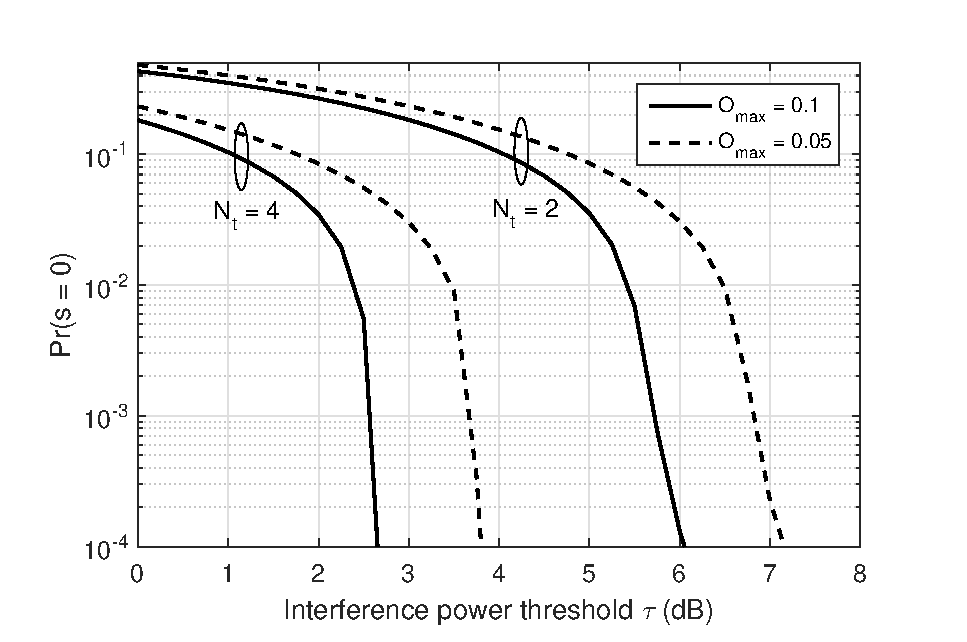
\includegraphics[width=\linewidth]{./Pr_s_0_vs_tau_pout_5_10_PT_5dB_Nt_2_4_Nr_2_M_4}
\caption{Probability of $s=\nx$ as a function of $\tau$ for different values of $\outmax$ and $\Nt$ ($\Pt = 5$~dB, $\Nr=2$, and QPSK).}
\label{fig:Pr_s_0_vs_tau}
\end{figure}



{\em Benchmarking:} We now compare the performance of LWIIR with the following rules considered in the literature. To ensure a fair comparison, these rules are adapted to enable them to meet the interference-outage constraint. 

\newcommand{\aicconst}{\nu}
\newcommand{\emiconst}{\beta}
\newcommand{\emslirconst}{\eta}
\newcommand{\epicconst}{\xi}
\newcommand{\enset}{{\cal{W}}}

\begin{enumerate}
\item {\em Enhanced Minimum Interference (EMI) Rule~\cite{Sarvendranath_2013_TCOM}}: Among the antennas $1,\ldots,\Nt$, it selects the one with the lowest STx-PRx channel power gain. However, it selects antenna $\nx$ when all the STx-PRx channel power gains exceed a threshold $\emiconst$. It is given by
\begin{equation}
\label{eq:MI_rule}
s = \left\{
\begin{array}{ll}
\nx, & \text{if}~ \gk{1}\geq\emiconst,\ldots,\gk{\Nt}\geq\emiconst,\\
\argmin\limits_{k\in\antopts}\{\gk{k}\}, &\text{otherwise}.  
\end{array}\right.
\end{equation} 


\item {\em Enhanced Maximum-Signal-Power to Leak-Interference-Power-Ratio (EMSLIR) Rule~\cite{Sarvendranath_2014_TCOM}}: Among the antennas $1,\ldots,\Nt$, it selects the one with the largest ratio of the STx-SRx sum channel power gain to the STx-PRx channel power gain. However, it selects antenna $0$ when these ratios of all the antennas are below a threshold $\emslirconst$.  It is given by
\begin{equation}
\label{eq:MSLIR_rule}
s = \left\{
\begin{array}{ll}
\nx,  \hspace{35pt}\text{if}~\frhg{1}\leq\emslirconst,&\!\!\!\!\ldots,\frhg{\Nt}\leq\emslirconst,\\
\argmax\limits_{k\in\{1,\ldots,\Nt\}}\left\lbrace \frhg{k}\right\rbrace, &\text{otherwise}.
\end{array}\right.
\end{equation} 


The thresholds $\emiconst$ of the EMI rule and $\emslirconst$ of the EMSLIR rules are chosen to ensure that the interference-outage constraint is met with equality in the interference-constrained region. Note that setting $\emiconst=\infty$ and $\emslirconst=0$ reduces the EMI and the EMSLIR rules to the MI and the MSLIR rules, respectively, in~\cite{Zhou_2008_IET}.

\item {\em Generalized HYA (GHYA) Rule}: Let $\enset = \{ k|\gk{k}\leq\epicconst,1\leq k\leq\Nt\}$ denote the set of all antennas whose STx-PRx channel power gains are below a threshold $\epicconst$. The GHYA rule selects the antenna $k$ with the largest $\sumnr\hk{ik}$ from $\enset$ or antenna $0$ if $\enset$ is empty. It is given by
\begin{equation}
\label{eq:GHYA_rule}
s = \left\{
\begin{array}{ll}
\nx, & \text{if}~\enset=\nullset,\\
\argmax\limits_{k\in \enset }\left\lbrace \sumnr\hk{ik} \right\rbrace, &\text{otherwise},  
\end{array}\right.
\end{equation} 
where $\epicconst$ is chosen such that interference-outage constraint is met with equality in the interference-constrained region. This reduces to the HYA rule for $\epicconst=\tau/\Pt$.

\item {\em Average Interference Constraint (AIC) Rule~\cite{Sarvendranath_2013_TCOM}}: It selects the antenna as follows
\begin{equation}
s = \argmin_{k\in\allopts} \left\lbrace \SEP(\bhk{k}) + \aicconst \gk{k}   \right\rbrace,
\end{equation}
where $\aicconst$ is chosen such that interference-outage constraint is met with equality in the interference-constrained region. It is optimal for the average interference constraint. 



\item {\em Difference Selection (DS) Rule~\cite{Wang_2011_TCom,Sarvendranath_2014_TCOM}}: Among antennas $1,\ldots,\Nt$, it selects the one that maximizes the weighted difference $\delta \sumnr\hk{ik} -(1-\delta) \gk{k} $, where, as above, $\delta \in [0, 1]$ is chosen to satisfy the interference-outage constraint.







\end{enumerate}


Figure~\ref{fig:BM_SEP_vs_tau} compares the average SEPs of all the above TAS rules. (i)~For $\itau < 15.6$~dB, LWIIR is in the interference-outage constrained region and outperforms all other rules. For example, at $\itau=12$~dB,  its average SEP is lower by a factor of $14.5$, $58.1$, $1.5$, $14.4$, and $9.2$ than the DS, EMI, AIC, GHYA, and EMSLIR  rules, respectively.  (ii)~For $\itau \geq 15.6$~dB, LWIIR is in the interference-outage unconstrained region. The average SEPs of the LWIIR, AIC, GHYA, and DS rules saturate to the same value because they reduce to  $\caluncons$, which does not depend on $\itau$. The average SEPs of EMI and EMSLIR also saturate, but to values that are 1-2 orders of magnitude larger. 



\begin{figure}
	\centering 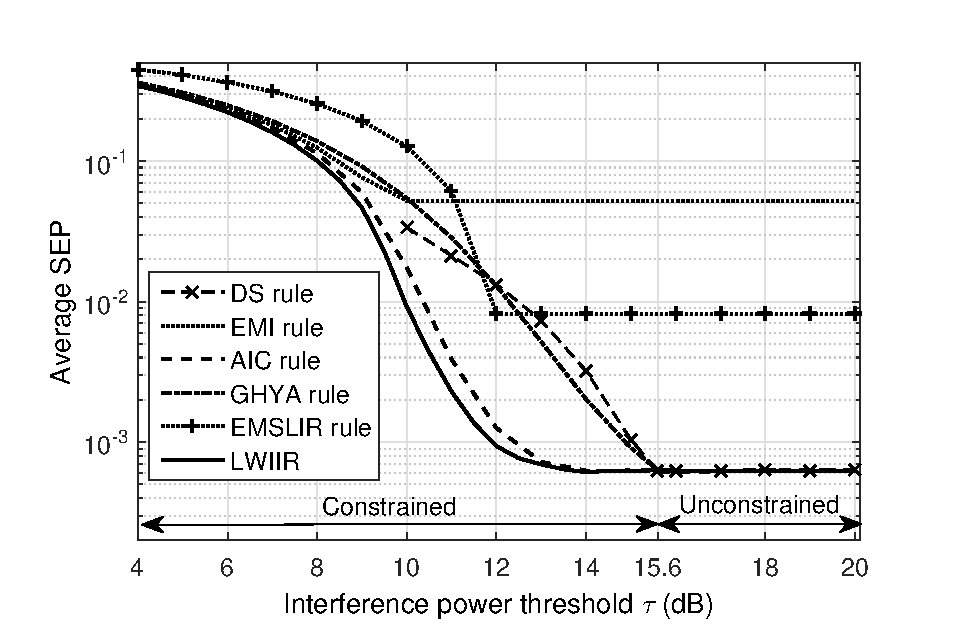
\includegraphics[width=\linewidth]{./BM_gs_SEP_vs_tau_pout_10_PT_12dB_Nt_4_M_4.eps}
	\caption{Performance benchmarking: Average SEPs of LWIIR and several TAS rules proposed in the literature ($\outmax = 0.1$, $\Pt = 12$~dB, $\Nt = 4$, $\Nr=1$, and QPSK).}
	\label{fig:BM_SEP_vs_tau}
\end{figure}


{\em Impact of Imperfect CSI:} Figures~\ref{fig:out_vs_tau_imp_CSI} and~\ref{fig:sep_vs_tau_imp_CSI} study the impact of imperfect CSI on the interference-outage probability and the average SEP, respectively, of LWIIR as a function of $\tau$. The scenarios with imperfect $\Hmx$ ($\hpilotpower=5$~dB and $\gpilotpower\tendsto\infty$) and imperfect $\g$ ($\hpilotpower\tendsto\infty$ and $\gpilotpower=5$~dB) are compared with the perfect CSI scenario. The analysis and  simulation results match in both figures. (i)~In the interference-outage constrained region ($\itau<13.6$~dB), the interference-outage probability with perfect CSI is exactly $\outmax=0.1$. However, with imperfect $\g$, it always exceeds  $\outmax$ because the probability of selecting an outage-incompatible antenna increases. This also results in a  lower average SEP compared to that for perfect CSI. Notably, the trends are different with imperfect $\Hmx$. Here, the interference-outage probability is below $\outmax$ for $\itau\leq10.6$~dB. Another difference is that the average SEP is always worse than that for perfect CSI. (ii)~In the interference-outage unconstrained region ($\itau \geq 13.6$~dB),  $\caluncons$ is the optimal TAS rule for all three cases. Therefore, the 
interference-outage probability becomes $\un$ for all cases. We also see that the average SEP with imperfect $\g$ saturates to the same value as that for perfect CSI. However, with imperfect $\Hmx$, it saturates to a higher value. With imperfect CSI, the other TAS rules also violate the interference-outage constraint, but by different extents.  The corresponding plots are not shown due to lack of space. 



\begin{figure}
	\centering
	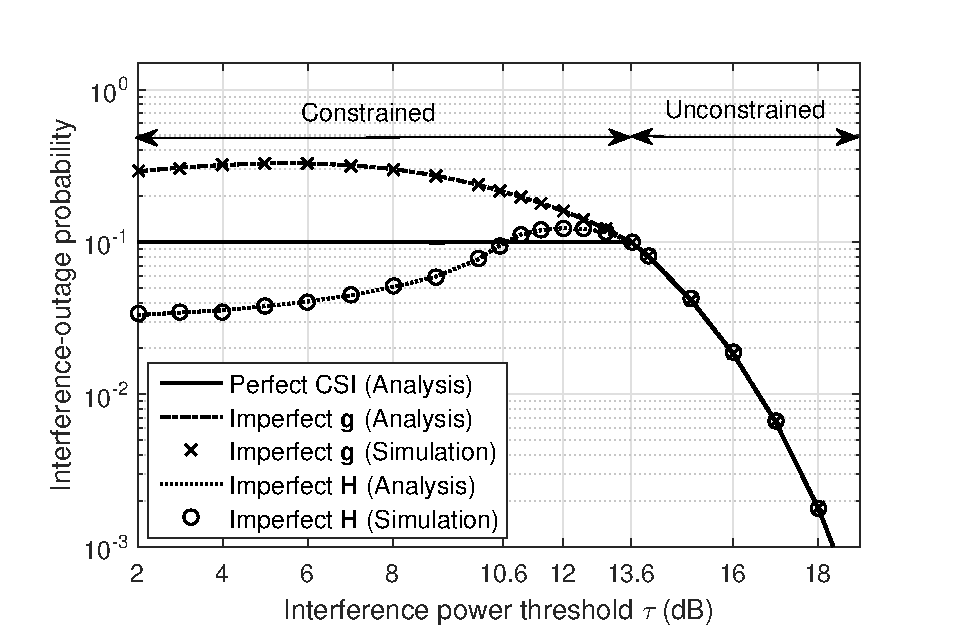
\includegraphics[width=\linewidth]{./Combined_outage_vs_tau_pout_10_PT_10dB_Nt_2_Nr_2_M_4.eps}
	\caption{Imperfect CSI: Interference-outage probability as a function of $\itau$ ($\outmax=0.1$, $\Pt = 10$~dB, $\Nt = 2$, $\Nr = 2$, and QPSK).}
	\label{fig:out_vs_tau_imp_CSI}
\end{figure}


\begin{figure}
	\centering 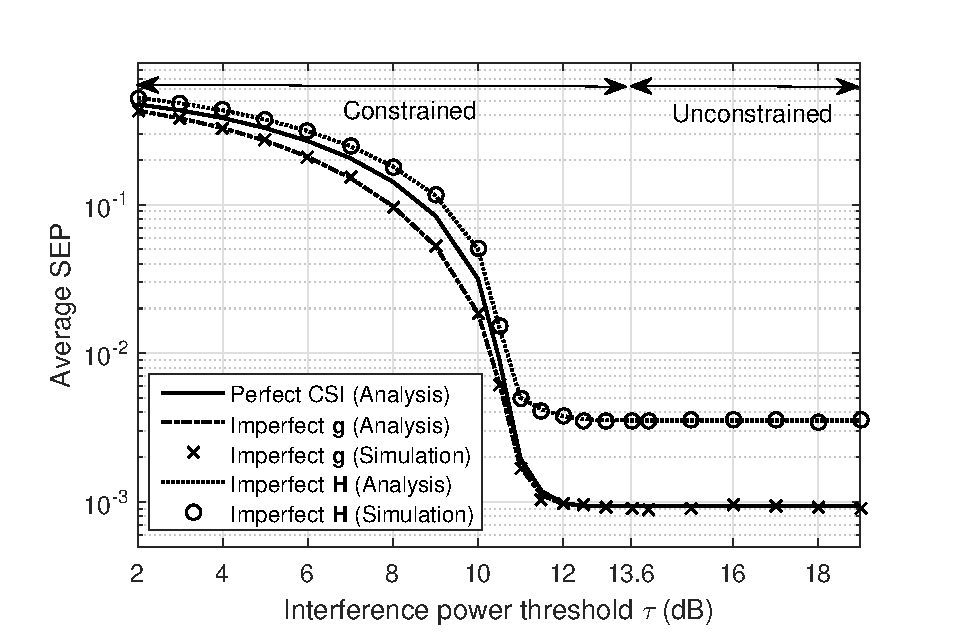
\includegraphics[width=\linewidth]{./Combined_SEP_vs_tau_pout_10_PT_10dB_Nt_2_Nr_2_M_4.eps}
	\caption{Imperfect CSI: Average SEP as a function of $\itau$ ($\outmax=0.1$, $\Pt = 10$~dB, $\Nt = 2$, $\Nr = 2$, and QPSK).}
	\label{fig:sep_vs_tau_imp_CSI}
\end{figure}


\section{Conclusions}
\label{sec:conclusions}
We proposed a novel and SEP-optimal TAS rule called LWIIR for an underlay CR system that is subject to the interference-outage constraint, which generalized the widely studied peak interference constraint. It applied to the general class of continuous fading models and to many constellations. LWIIR was a discontinuous function of the STx-PRx channel power gain and was different from the TAS rules proposed in the literature. We derived a general expression for the average SEP of LWIIR for an arbitrary number of transmit and receive antennas. LWIIR reduced the SEP significantly  compared to the other TAS rules. Furthermore, we saw that imperfect CSI of the STx-SRx channel power gains and of the STx-PRx channel power gains had different impacts on the interference-outage probability and the average SEP. 

Several interesting avenues for research arise out of this work.  These include incorporating multiple primary receivers, antenna subset selection, and continuous power control in the model to better utilize the available CSI. Secondly, it would be of interest to develop the optimal TAS rule when the STx has imperfect CSI. Lastly, a comprehensive  system-level study that characterizes  and compares the impact of the  different interference constraints on the primary system as well as  the secondary system is desirable.



\appendix
\subsection{Proof of Lemma~\ref{lem:outage_Nt}}
\label{proof:outage_Nt}
We first derive the expression for $\outlam = \prob{\gkgrtaubyptinl{s}}$ in~\eqref{eq:pr_outage_ccdf}. $\Pt \gk{s}$ can exceed  $\itau$ only when $s\neq0$. Thus, using the law of total probability, $\outlam$ is given by
%
\begin{equation}
\outlam =  \sum_{\eqidx=1}^{\Nt}\text{Pr}\brac{s=\eqidx,\gkgrtaubypt{\eqidx}}
=\Nt\text{Pr}\brac{s=1,\gkgrtaubypt{1}}.
\label{eq:out_1}
\end{equation}
%
The second equality above follows due to symmetry.

Let $k$ antennas out of the antennas $2,\ldots,\Nt$ be outage-compatible. The total number of ways in which such $k$ antennas can be chosen is $\nck{\Nt-1}{k}$. Given $k$, all these combinations are equally likely as the STx-PRx channels are i.i.d. One such combination is when the antennas $2,\ldots,k+1$ are outage-compatible. For it, define the event   $\setAk=\left(\gklttaubyptinl{2}\right)\cap\cdots\cap\left(\gklttaubyptinl{k+1}\right)\cap\left( \gkgrtaubyptinl{k+2}\right)\cap\cdots\cap\left(\gkgrtaubyptinl{\Nt}\right)$. Therefore, using the law of total probability, we can write $\outlam$ in~\eqref{eq:out_1} as
%
\begin{align}
\outlam &=\Nt\sum_{k=0}^{\Nt-1}\nck{\Nt-1}{k} \text{Pr}\brac{s = 1,\gkgrtaubypt{1},\setAk}, \\
&=\Nt\sum_{k=0}^{\Nt-1}\nck{\Nt-1}{k}  \text{Pr}\brac{\setGk} \text{Pr}\brac{s = 1\Given \setGk},
\label{eq:out_3}
\end{align}
%
where $\setGk$ denotes the event  $\left(\gkgrtaubyptinl{1}\right)\cap\setAk $. As $\gk{1},\ldots,\gk{\Nt}$ are i.i.d., we get 
%
\begin{equation}
\label{eq:pr_Gk}
\prob{\setGk} = \left(1-\un\right)^k\un^{\Nt-k}.
\end{equation}
%

{\em Expression for $\prob{s = 1\Given\setGk}$:} Given $\setGk$, $\callamrule$ in~\eqref{eq:lam_weight_rule} selects antenna 1 if $\ykplambym{1}<\yk{i}$ for $2\leq i \leq k+1$,  $\ykplambym{1}<\ykplambym{j}$ for $k+2\leq j \leq \Nt$, and $\ykplambym{1}<\yk{0}=1$.  Hence,
%
%\begin{align}
%\label{eq:out_5}
%\text{Pr}\!\left(\!s\! = \! 1 \! \Given \! \setGk \right)\!\!=&\text{Pr}\!\left(\!\xplambymcomp \! < \! 1, \xplambymcomp \!<\! \yk{2},\! \ldots,\xplambymcomp\!<\!\yk{k+1},
%\right. \nonumber\\
%&\!\left.\xplambymcomp\!<\!\ykplambymcomp{k+2}\!,\! \ldots\!,\xplambymcomp \!<\! \ykplambymcomp{\Nt}\!\Given\!\setGk\!\right)\!.
%\end{align} 
%
\begin{align}
\label{eq:out_5}
\text{Pr}\left(s =  1  \Given  \setGk \right)=&\text{Pr}\left(\xplambymcomp  <  1, \xplambymcomp < \yk{2},\ldots, \right. \nonumber\\
&\quad\xplambymcomp<\yk{k+1},
\xplambymcomp<\ykplambymcomp{k+2}, \nonumber\\
&\quad\left. \ldots,\xplambymcomp < \ykplambymcomp{\Nt}\Given\setGk\right).
\end{align}

Conditioning on $\yk{1}$, the events in~\eqref{eq:out_5} are mutually independent. Furthermore, $\yk{2},\ldots,\yk{\Nt} $ are identically distributed. Hence, we get
%
\begin{multline}
\text{Pr}\brac{s=1\Given \setGk, \yk{1}=x}\!=\! \indic{x<1-\lambycone}\!\!\left[\text{Pr}\brac{\yk{2}\!>\!x+\lambycone}\right]^{k} \\\times \left[\text{Pr}\brac{\yk{k+2}>x}\right]^{\Nt-k-1}.
\label{eq:out_6}
\end{multline}
%
Now, averaging over $\yk{1}$ and writing it in terms of the CCDF and the PDF of $\yk{1}$, we get 
\begin{multline}
\!\!\!\text{Pr}\brac{s=1\Given\setGk} =\!\int_{0}^{1-\lambycone}\!\!\left[F_{y}^{c}\left(x+\lambycone\right)\right]^{k} \left[F_{y}^{c}\left(x\right)\right]^{\Nt-k-1}\\\times f_{y}(x)\,dx.
\label{eq:out_7}
\end{multline}
Finally, substituting~\eqref{eq:out_7} in~\eqref{eq:out_3} yields~\eqref{eq:pr_outage_ccdf}. 

{\em Existence of $\lam$}: From~\eqref{eq:pr_outage_ccdf}, we see that for the class of continuous fading models, $\outlam$ is a continuous and strictly decreasing  function in $\lam$. Furthermore, $\outlam=\un$ when $\lam=0$ and $\outlam=0$ when $\lam=\cone$. Thus, by the intermediate value theorem, for every $0\leq\outmax\leq\un$,  there exists a corresponding unique $\lam\in[0,\cone]$ such that $\outlam=\outmax$. 
  



\subsection{Proof of Result~\ref{res:selection_rule_on_off}}
\label{proof:selection_rule_on_off}

We consider the following two cases.

{ 1. $\outmax\geq\un$:} From the discussion in Comment 1 in Section~\ref{sec:lambda_rule}, it follows that the interference unconstrained rule $\caluncons$ is clearly the optimal rule. 

{2. $0\leq\outmax<\un$:} Here, $\caluncons$ does not satisfy the interference-outage constraint. Instead, consider $\callamstarrule$ in~\eqref{eq:lam_weight_rule}, where $\lamstar$ is chosen such that the interference-outage probability is equal to $\outmax$. From Lemma~\ref{lem:outage_Nt}, such a choice of $\lamstar$ exists and is positive. For a given realization of $\yk{1},\ldots,\yk{\Nt}$ and $\gk{1},\ldots,\gk{\Nt}$,   $\callamstarrule$ selects the antenna $\sstar$ that minimizes $\yk{k} + \left( {\lamstar}/{\cone}\right) \gindicinl{k}$, for $0\leq k\leq\Nt$.  Consider any TAS rule $\asrule$ that selects the antenna  $s=\phi(\Hmx,\g)$ and satisfies the interference-outage constraint.\footnote{We do not denote the antennas selected by $\callamstarrule$ and $\phi$ as $s^*(\Hmx,\g)$ and $s(\Hmx,\g)$ in order to keep the notation simple.} 

From above, it follows that   
\begin{equation}
\label{eq:opt_rul_1}  
   \explow{\Hmx,\g}{\yk{{\sstar}} + \frac{\lamstar}{\cone}\gindic{{\sstar}}} \leq  \explow{\Hmx,\g}{\yk{{s}} + \frac{\lamstar}{\cone}\gindic{{s}}}.
\end{equation}
%
%
Using $\explow{\Hmx,\g}{\gindicinl{k}}=\prob{\gkgrtaubyptinl{k}}$ and
substituting $\yk{k}={\SEP(\bhk{k})}/{\cone}$ (from~\eqref{eq:yi_def}), we get
%
\begin{multline}
\label{eq:opt_rul_2}
   \explow{\Hmx,\g}{\SEP(\hsstar)} + \lamstar \, \prob{\gkgrtaubypt{\sstar}} \\\leq  \explow{\Hmx,\g}{\SEP(\hs)} + \lamstar \, \prob{\gkgrtaubypt{s}}.
\end{multline}
%
We also know that $\prob{\gkgrtaubyptinl{\sstar}}=\outmax$. Rearranging terms, we get
%
\begin{multline}
\label{eq:ineq_3}
\explow{\Hmx,\g}{\SEP(\hsstar)} \leq \explow{\Hmx,\g}{\SEP(\hs)}\\ + \lamstar \left( \prob{\gkgrtaubypt{s}} -  \outmax \right).
\end{multline}
%
As $\phi$ satisfies the interference-outage constraint and $\lamstar>0$,~\eqref{eq:ineq_3} implies that $\explow{\Hmx,\g}{\SEP(\hsstar)} \leq \explow{\Hmx,\g}{\SEP(\hs)}$. Thus, $\callamstarrule$ is optimal.




\subsection{Proof of Result~\ref{thm:SEP_exact_Nt_gen}}
\label{proof:SEP_exact_Nt_gen}
We start with the probability of error conditioned on $\y \define [\yk{1},\ldots,\yk{\Nt}]$, which we denote by $\prob{\Err \given \y}$. Using the law of total probability, it can be written as
%\g
\begin{equation}
\prob{\Err \given \y} =  \prob{s=\nx,\Err\given\y} + \sum_{k=1}^{\Nt}\prob{s=k,\Err\given\y}.
\label{eq:Perr_all_h}
\end{equation}
%
Furthermore, $\prob{s\!=\!k,\Err\given\y}\!=\!\prob{s\!=\!k\given\y} \prob{\Err\given\y,s=k}$, for $0\leq k \leq \Nt$. Averaging over $\y$  and exploiting symmetry, $\avgSEP$ is given by
\begin{multline}
\label{eq:avg_SEP_1}
 \avgSEP = \explow{\y}{\prob{s=\nx\given\y}\prob{\Err\given\y,s=\nx}} \\+ \Nt\explow{\y}{\prob{s=1\given\y}\prob{\Err\given\y,s=1}}.
\end{multline}

Given $s=0$, the SEP is equal to $\zerosep$. Thus, 
\begin{equation}
\prob{\Err\given\y,s=\nx}=\SEP\left(\bhk{0}\right)=\zerosep.
\end{equation}
Given $s=1$,  from~\eqref{eq:yi_def}, we get 
\begin{equation}
\prob{\Err\given\y,s=1}=\SEP\left(\bhk{1}\right) =\cone \yk{1}.
\end{equation}
Hence,
%
\begin{equation}
\label{eq:avg_SEP_3}
\avgSEP  = \zerosep \explow{\y}{\prob{s=\nx\given\y}} + \Nt\cone\explow{\y}{\yk{1}\prob{s=1\given\y}}.
\end{equation}
%
From the law of total expectation, we know that $\explow{\y}{\prob{s=\nx\given\y}} = \prob{s = 0}$.
Similarly, 
\begin{equation}
\label{eq:avg_sep_3_one}
\explow{\y}{\yk{1}\prob{s = 1\given \y} } = \explow{\yk{1}}{\yk{1} \prob{s = 1\given \yk{1}}  }.
\end{equation}

Substituting these two results into~\eqref{eq:avg_SEP_3}, we get $\avgSEP  = \termone + \termtwo$,
%
where 
\begin{align}
\termone &=\zerosep \prob{s = 0},\\
\termtwo &=\Nt\cone \explow{\yk{1}}{ \yk{1}\prob{s = 1\given \yk{1}} }. 
\end{align}
%
We now evaluate $\termone$ and $\termtwo$.

{\em First Term $\termone$:}
From~\eqref{eq:lam_weight_rule}, we know that ${s=0}$ is selected when the selection metrics of antennas $1,\ldots,\Nt$ exceed the selection metric of antenna $0$, which is $\yk{0}=1$. This happens only when antennas $1,\ldots,\Nt$ are all outage-incompatible. Therefore, we can write
\begin{multline}
\termone =  \zerosep \text{Pr}\left(  \gk{1}>\taubypt,\dots,\gk{\Nt}>\taubypt, \right. \\ \left. \yk{1}+\lambycone >1,\ldots,\yk{\Nt}+\lambycone >1\right).
\label{eq:termone_a}
\end{multline}
%
Using the fact that channels are i.i.d., and by writing the above formula in terms of the CCDFs of $\yk{1}$ and $\gk{1}$, we get the first term in~\eqref{eq:SEP_Nt_gen}.


{\em Second Term $\termtwo$}: From the law of total probability, we have 
%
\begin{multline}
\prob{s = 1\given \yk{1}} = \prob{s = 1,\gkgrtaubypt{1}\Given\yk{1}} \\ + \prob{s = 1,\gklttaubypt{1}\Given \yk{1}}. 
\label{eq:pr_s_1}
\end{multline}
%
We recall  the definition of the events $\setAk$ and   $\setGk=\left(\gkgrtaubyptinl{1}\right)\cap\setAk$ from Appendix~\ref{proof:outage_Nt}. Similarly, we define the event $\setLk\define\left(\gklttaubyptinl{1}\right)\cap\setAk $. Summing over all the events in which $k$ antennas out of the antennas $2,\ldots,\Nt$ are outage-compatible, we get the following in a manner similar to~\eqref{eq:out_3}:
\begin{align}
\prob{s = 1\given \yk{1}}  =& \sum_{k=0}^{\Nt-1}\nck{\Nt-1}{k}
 \prob{s = 1 \Given \setGk, \yk{1}} \prob{\setGk}\nonumber \\
 &+ \sum_{k=0}^{\Nt-1}\!\!\nck{\Nt-1}{k} \prob{s = 1 \Given \setLk, \yk{1}} \prob{\setLk}. 
\label{eq:pr_s_1_2}
\end{align}
% 
%
The expression for $\prob{s = 1\given \setGk, \yk{1}}$ is given in~\eqref{eq:out_6}.  The expression for $\prob{s = 1\given \setLk, \yk{1}}$ can be derived along lines similar to that for $\prob{s = 1\given \setGk, \yk{1}}$ in~\eqref{eq:out_6}. This yields   
\begin{align}
\!\text{Pr}\brac{\s =1\given \setLk,\yk{1}=x} =&\indic{x\leq\lambycone} \left[ F_{y}^{c}\brac{x}\right]^{k} +\indic{x>\lambycone}\nonumber\\&\times\!\left[ F_{y}^{c}\brac{x}\right]^{k}\!\left[ F_{y}^{c}\brac{x-\lambycone}\right] ^{\!\Nt-k-1}.
\label{eq:prob_gklt}
\end{align}
%
Substituting $\prob{\setGk} = \left(1-\un\right)^k\un^{\Nt-k}$ and~\eqref{eq:out_6} in~\eqref{eq:pr_s_1_2} simplifies the first part of~\eqref{eq:pr_s_1_2}. Similarly, substituting $\prob{\setLk}=\left(1-\un\right)^{k+1}\un^{\Nt-k-1}$ and~\eqref{eq:prob_gklt} simplifies the second part of~\eqref{eq:pr_s_1_2}. Substituting~\eqref{eq:pr_s_1_2} in $\explow{\yk{1}}{ \yk{1}\prob{s = 1\given \yk{1}}}$ and averaging over $\yk{1}$ yields~\eqref{eq:termtwo_gen}. 


\subsection{Brief Proof of Result~\ref{thm:avg_SEP_imperfect}}
\label{proof:avg_SEP_imperfect_CSI}
The antenna $s$ selected by $\callamrule$  now depends on $\yhatvec\define\left[\ykhat{1},\ldots,\ykhat{\Nt} \right]$, while the SEP using the antenna $k$ is given by $\cone\yk{k}$, for $1\leq k\leq\Nt$.  Hence, to analyze the average SEP, we instead condition on $\y$ and  $\yhatvec$ as follows:
%
\begin{equation}
\prob{\Err \given \y,\yhatvec} =  \prob{s=\nx,\Err\given \y, \yhatvec} + \sum_{k=1}^{\Nt}\prob{s=k,\Err\given\y,\yhatvec}.
\label{eq:Perr_all_imp_csi}
\end{equation} 
%
Simplifying further in a manner similar to the steps from~\eqref{eq:Perr_all_h} to~\eqref{eq:avg_sep_3_one} in Appendix~\ref{proof:SEP_exact_Nt_gen}, we get
%
\begin{equation}
\label{eq:avg_SEP_3_IMP_CSI}
\avgSEP = \zerosep \prob{s=\nx} + \Nt\cone\explow{\yk{1},\ykhat{1}}{\yk{1}\prob{s=1\given \ykhat{1}}}.
\end{equation}
%

The first term in~\eqref{eq:avg_SEP_3_IMP_CSI} can be obtained by replacing $\gk{k}$ with $\gkhat{k}$ and $\yk{k}$ with $\ykhat{k}$ in~\eqref{eq:termone_a}. The expectation in the second term can be written in terms of the joint PDF $f_{\yk{1},\ykhat{1}}\left(\cdot,\cdot\right)$ of the correlated RVs $\yk{1}$ and $\ykhat{1}$ as follows:
%
\begin{align}
\label{eq:avg_SEP_4_IMP_CSI}
\explow{\yk{1},\ykhat{1}}{\yk{1}\prob{s=1\given \ykhat{1}}}= &\int_{\xhat=0}^{1} \prob{s=1\given \ykhat{1}=\xhat} \nonumber\\
&\times\left[ \int_{x=0}^{1}  x  f_{\yk{1},\ykhat{1}}\left(x,\xhat\right)dx\right] d\xhat.
\end{align}
%
The expression for $\prob{s=1\given\ykhat{1}=\xhat}$ can be derived along lines similar to the steps from~\eqref{eq:pr_s_1} to~\eqref{eq:prob_gklt} in Appendix~\ref{proof:SEP_exact_Nt_gen}, by replacing $\yk{1}$ with $\ykhat{1}$ and $\gk{1}$ with $\gkhat{1}$. Thus, its final expression is obtained by replacing $\ccdfyrv{\cdot}$ with $\ccdfyhatrv{\cdot}$ and $\un$  with $\unhat$ in the expression for  $\prob{s=1\given\yk{1}}$ in~\eqref{eq:pr_s_1_2}. 

{\em Joint PDF $f_{\yk{1},\ykhat{1}}\left(\cdot,\cdot\right)$:} Consider first the joint PDF of two bivariate gamma RVs $V\define\sumnr\hk{i1}$ and $W\define\sumnr\hkhat{i1}$, which is given by~\cite[eq. (6.1)]{simon_alouini_book}
\begin{align}
\label{eq:bivargammaPDF}
\!f_{V,W}(v,w) = & \frac{\exp\left[{-\frac{1}{(1-\rhoh)}\left( \frac{v}{\muh}+\frac{w}{\muhhat}\right) } \right]}{(\Nr-1)! \left(1-\rhoh \right)\muh\muhhat }\left(\frac{vw}{\rhoh \muh\muhhat}\right)^{\frac{\Nr-1}{2}} \nonumber\\
&\times I_{\Nr-1}\left(\frac{2\sqrt{\rhoh vw}}{(1-\rhoh)\sqrt{\muh\muhhat}}\right)\!,~v, w \geq 0.
\end{align}
%  
Here, $I_{\Nr-1}\left(\cdot \right) $ is the modified Bessel function of $(\Nr-1)^{\text{th}}$ order. From it, we can obtain the joint PDF $f_{\yk{1},\ykhat{1}}\left(\cdot,\cdot\right)$ using the variable transformation $\yk{1}=\exp\left(-\Pt V/(\ctwo\noisevar)\right)$ and $\ykhat{1}=\exp\left(-\Pt W/(\ctwo\noisevar) \right)$, with $\yk{1}$ given by~\eqref{eq:yi_def} and $\ykhat{1}$ by~\eqref{eq:yihat_def}.  
We can then show that 
%
\begin{equation}
\label{eq:y1_jpdf}
\int_{0}^{1} x f_{\yk{1}\ykhat{1}}\left(x,\xhat\right)\,dx = \frac{\T^{\Nr}\left(-\ln\left({\xhat} \right)\right)^{\Nr-1}\xhat^{\D}}{(\Nr-1)!},
\end{equation}
where $\T$ and $\D$ are defined in the result statement. Substituting~\eqref{eq:y1_jpdf}  in~\eqref{eq:avg_SEP_4_IMP_CSI} and then in~\eqref{eq:avg_SEP_3_IMP_CSI}  yields~\eqref{eq:avg_SEP_imperfect}.



\subsection{Proof of Result~\ref{thm:outage_imperfect_CSI}}
\label{proof:outage_imperfect_CSI}
Instead of~\eqref{eq:out_1}, we write the outage probability as follows: 
\begin{multline}
\outlam= \Nt\text{Pr}\brac{s=1,\gkgrtaubypt{1},\gkhatlttaubypt{1}}  \\+ \Nt\text{Pr}\brac{s=1,\gkgrtaubypt{1},\gkhatgrtaubypt{1}}.
\label{eq:outhat_2}
\end{multline}
Let $k$ be the number of STx antennas for which $\gkhatlttaubyptinl{j}$, for $2\leq j \leq\Nt$. Similar to the events $\setAk$, $\setLk$,  and  $\setGk$ that were defined in Appendices~\ref{proof:outage_Nt} and~\ref{proof:SEP_exact_Nt_gen}, we define $\setAkhat=\left(  \gkhatlttaubyptinl{2}\right)\cap\cdots\cap\left(\gkhatlttaubyptinl{k+1}\right)\cap\left(\gkhatgrtaubyptinl{k+2}\right)\cap\dots\cap\left(\gkhatgrtaubyptinl{\Nt}\right)$, $\setLkhat\define\left(\gkhatlttaubyptinl{1}\right)\cap\setAkhat$, and $\setGkhat\define\left(\gkhatgrtaubyptinl{1}\right)\cap\setAkhat$. Then, along lines similar to~\eqref{eq:pr_s_1_2}, we can write the first term in~\eqref{eq:outhat_2}  as
%
\begin{align}
&\text{Pr}\brac{s=1,\gkgrtaubypt{1},\gkhatlttaubypt{1}}  =\nonumber\\
&\quad\quad\sum_{k=0}^{\Nt-1}\nck{\Nt-1}{k}
\prob{\gkgrtaubypt{1},\setLkhat}\nonumber\\
&\quad\quad\times\text{Pr}\brac{s = 1 \Given \gkgrtaubypt{1},\setLkhat}. 
\label{eq:pr_s_1_2_imp}
\end{align}

To compute this, we proceed as follows:

1) Given $\gkhatlttaubyptinl{1}$ and the definition of $s$ in~\eqref{eq:shat}, it follows that the selection of antenna 1 does not depend on $\gk{1}$. Thus, $\prob{s = 1 \Given \gkgrtaubyptinl{1},\setLkhat}=\prob{s = 1 \Given \setLkhat}$, which is obtained by replacing $\yk{1}$ with $\ykhat{1}$ and $\ccdfyrv{\cdot}$ with $\ccdfyhatrv{\cdot}$ in~\eqref{eq:prob_gklt} and then averaging over $\ykhat{1}$. 

2) Using the fact that $\gkhat{2},\ldots\gkhat{\Nt}$ are independent of $\gk{1}$ and $\gkhat{1}$, we get  
%
\begin{equation}
\prob{\gkgrtaubypt{1},\setLkhat} =\prob{\gkgrtaubypt{1},\gkhatlttaubypt{1}}\prob{\setAkhat}. 
\end{equation}
%
Furthermore, since $\gkhat{2},\ldots,\gkhat{\Nt}$ are i.i.d., we get $\prob{\setAkhat}=\left(1- \unhat \right)^{k} \unhat^{\Nt-k-1}$. Also,
\begin{equation}
\label{eq:g1_integral}
\Probglt\define\prob{\!\gkgrtaubypt{1}\!,\gkhatlttaubypt{1}\!}\!\!=\!\!\int_{0}^{\taubypt}\!\!\!\int_{\taubypt}^{\infty}\!\!f_{\gk{1},\gkhat{1}}\!\left(x,\xhat \right)dx\, d\xhat,
\end{equation}
where $f_{\gk{1},\gkhat{1}}\left(\cdot,\cdot \right)$ is the joint PDF of the bivariate exponential RVs $\gk{1}$ and $\gkhat{1}$.  This is a special case of~\eqref{eq:bivargammaPDF} with $\Nr=1$, and is obtained by replacing $\muh$, $\muhhat$, and $\rhoh$ with $\mug$, $\mughat$, and $\rhog$, respectively. Then, evaluating the above integral yields the expression for $\Probglt$ in the result statement.


The second term in~\eqref{eq:outhat_2} can be simplified in a similar manner. Substituting the expressions for these two probability terms in~\eqref{eq:outhat_2} yields~\eqref{eq:pr_outage_impefect}.
 



\begin{thebibliography}{10}
	\bibitem{Sarvendranath_2017_globecom}
	R.~Sarvendranath and N.~B. Mehta, ``Optimal transmit antenna selection rule for
	interference-outage constrained underlay {CR},'' in \emph{Proc.\ Globecom},
	Dec. 2017, pp. 1--6.
	
	\bibitem{Goldsmith_2009_PIEEE}
	A.~Goldsmith, S.~A. Jafar, I.~Maric, and S.~Srinivasa, ``Breaking spectrum
	gridlock with cognitive radios: An information theoretic perspective,''
	\emph{Proc.\ IEEE}, vol.~97, no.~5, pp. 894--914, May 2009.
	
	\bibitem{Fakhan_2014_TSP}
	F.~A. Khan, K.~Tourki, M.~S. Alouini, and K.~A. Qaraqe, ``Performance analysis
	of a power limited spectrum sharing system with {TAS/MRC},'' \emph{IEEE
		Trans.\ Signal Process.}, vol.~62, no.~4, pp. 954--967, Feb. 2014.
	
	\bibitem{Hanif_2015_globecom}
	M.~Hanif, H.~C. Yang, and M.~S. Alouini, ``Transmit antenna selection for
	underlay cognitive radio with instantaneous interference constraint,'' in
	\emph{Proc.\ Globecom}, Dec. 2015, pp. 1--5.
	
	\bibitem{Wang_2010_TWC}
	H.~Wang, J.~Lee, S.~Kim, and D.~Hong, ``Capacity enhancement of secondary links
	through spatial diversity in spectrum sharing,'' \emph{IEEE Trans.\ Wireless
		Commun.}, vol.~9, no.~2, pp. 494--499, Feb. 2010.
	
	\bibitem{RZhang_2009_TWC}
	R.~Zhang, ``On peak versus average interference power constraints for
	protecting primary users in cognitive radio networks,'' \emph{IEEE Trans.\
		Wireless Commun.}, vol.~8, no.~4, pp. 2112--2120, Apr. 2009.
	
	\bibitem{Suraweera_2010_TVT}
	H.~A. Suraweera, P.~J. Smith, and M.~Shafi, ``Capacity limits and performance
	analysis of cognitive radio with imperfect channel knowledge,'' \emph{IEEE
		Trans.\ Veh.\ Technol.}, vol.~59, no.~4, pp. 1811--1822, Feb. 2010.
	
	\bibitem{li_2011_pimrc}
	L.~Li, P.~I. Derwin, and M.~Pesavento, ``Symbol error rate analysis in
	multiuser underlay cognitive radio systems,'' in \emph{Proc.\ {PIMRC}}, Sep.
	2011, pp. 681--684.
	
	\bibitem{Sarvendranath_2013_TCOM}
	R.~Sarvendranath and N.~B. Mehta, ``Antenna selection in
	interference-constrained underlay cognitive radios: {SEP}-optimal rule and
	performance benchmarking,'' \emph{IEEE Trans.\ Commun.}, vol.~61, no.~2, pp.
	496--506, Feb. 2013.
	
	\bibitem{Sarvendranath_2014_TCOM}
	R.~Sarvendranath and N.~B. Mehta, ``Antenna selection with power adaptation in interference-constrained cognitive radios,'' \emph{IEEE Trans.\ Commun.}, vol.~62, no.~3, pp.
	786--796, Mar. 2014.
	
	\bibitem{Wang_2011_TCom}
	Y.~Wang and J.~Coon, ``Difference antenna selection and power allocation for
	wireless cognitive systems,'' \emph{IEEE Trans.\ Commun.}, vol.~59, no.~12,
	pp. 3494--3503, Dec. 2011.
	
	\bibitem{Kashyap_2014_TCOM}
	S.~Kashyap and N.~B. Mehta, ``Optimal binary power control for underlay {CR}
	with different interference constraints and impact of channel estimation
	errors,'' \emph{IEEE Trans.\ Commun.}, vol.~62, no.~11, pp. 3753--3764, Nov.
	2014.
	
	\bibitem{Sboui_2013_TWC}
	L.~Sboui, Z.~Rezki, and M.~S. Alouini, ``A unified framework for the ergodic
	capacity of spectrum sharing cognitive radio systems,'' \emph{IEEE Trans.\
		Wireless Commun.}, vol.~12, no.~2, pp. 877--887, Feb. 2013.
	
	\bibitem{mehta_2012_ComMag}
	N.~B. Mehta, S.~Kashyap, and A.~F. Molisch, ``Antenna selection in {LTE}: From
	motivation to specification,'' \emph{IEEE Commun.\ Mag.}, vol.~50, no.~10,
	pp. 144--150, Oct. 2012.
	
	\bibitem{Kong_2011_JCN}
	H.~Y. Kong and Asaduzzaman, ``On the outage behavior of interference
	temperature limited {CR-MISO} channel,'' \emph{J.\ Commun.\ Netw.}, vol.~13,
	no.~5, pp. 456--462, Oct. 2011.
	
	\bibitem{Peng_2016_eurasip}
	P.~Lan, L.~Chen, G.~Zhang, and F.~Sun, ``Performance analysis of transmit
	antenna selection for cognitive radio systems with imperfect channel
	estimation,'' \emph{EURASIP {J.} Adv. Signal Process.}, vol. 2016, no.~1,
	p.~72, Jun. 2016.
	
	\bibitem{musavian_2009_tcom}
	L.~Musavian and S.~Aissa, ``Fundamental capacity limits of cognitive radio in
	fading environments with imperfect channel information,'' \emph{IEEE Trans.\
		Commun.}, vol.~57, no.~11, pp. 3472--3480, Nov. 2009.
	
	\bibitem{das_2015_twc}
	P.~Das, N.~B. Mehta, and G.~Singh, ``Novel relay selection rules for average
	interference-constrained cognitive {AF} relay networks,'' \emph{IEEE Trans.\
		Wireless Commun.}, vol.~14, no.~8, pp. 4304--4315, Aug. 2015.
	
	\bibitem{Zhang_2017_tcom}
	L.~Zhang, G.~Zhao, W.~Zhou, L.~Li, G.~Wu, Y.~C. Liang, and S.~Li, ``Primary
	channel gain estimation for spectrum sharing in cognitive radio networks,''
	\emph{IEEE Trans.\ Commun.}, vol.~65, no.~10, pp. 4152--4162, Oct. 2017.
	
	\bibitem{Zhao_2008_TSP}
	Q.~Zhao, S.~Geirhofer, L.~Tong, and B.~M. Sadler, ``Opportunistic spectrum
	access via periodic channel sensing,'' \emph{IEEE Trans.\ Signal Process.},
	vol.~56, no.~2, pp. 785--796, Feb. 2008.
	
	\bibitem{RZhang_2008_DSAN}
	R.~Zhang and Y.~C. Liang, ``Exploiting hidden power-feedback loops for
	cognitive radio,'' in \emph{Proc.\ DySPAN}, Oct. 2008, pp. 1--5.
	
	\bibitem{Chung_2001_TCom}
	S.~T. Chung and A.~Goldsmith, ``Degrees of freedom in adaptive modulation: {A}
	unified view,'' \emph{IEEE Trans.\ Commun.}, vol.~49, pp. 1561--1571, Sep.
	2001.
	
	\bibitem{Kashyap_2013_TWC}
	S.~Kashyap and N.~B. Mehta, ``{SEP}-optimal transmit power policy for peak
	power and interference outage probability constrained underlay cognitive
	radios,'' \emph{IEEE Trans.\ Wireless Commun.}, vol.~12, no.~12, pp.
	6371--6381, Dec. 2013.
	
	\bibitem{abramowitz_stegun}
	M.~Abramowitz and I.~Stegun, \emph{Handbook of Mathematical Functions with
		Formulas, Graphs, and Mathematical Tables}, 9th~ed.\hskip 1em plus 0.5em
	minus 0.4em\relax Dover, 1972.
	
	\bibitem{Xiang_2012_SIAM}
	S.~Xiang and F.~Bornemann, ``On the convergence rates of {Gauss} and
	{Clenshaw}--{Curtis} quadrature for functions of limited regularity,''
	\emph{SIAM J. Numer. Anal.}, vol.~50, no.~5, pp. 2581--2587, 2012.
	
	\bibitem{CLRS_algo_book}
	T.~H. Cormen, C.~E. Leiserson, R.~L. Rivest, and C.~Stein, \emph{Introduction
		to Algorithms}, 3rd~ed.\hskip 1em plus 0.5em minus 0.4em\relax MIT Press,
	2009.
	
	\bibitem{gradshteyn00_book}
	L.~S. Gradshteyn and L.~M. Ryzhik, \emph{Tables of Integrals, Series and
		Products}.\hskip 1em plus 0.5em minus 0.4em\relax Academic Press, 2000.
	
	\bibitem{Kashyap_2015_wicomlet}
	S.~Kashyap and N.~B. Mehta, ``Power gain estimation and its impact on binary
	power control in underlay cognitive radio,'' \emph{IEEE Wireless Commun.\
		Lett.}, vol.~4, no.~2, pp. 193--196, Apr. 2015.
	
	\bibitem{simon_alouini_book}
	M.~Simon and M.-S. Alouini, \emph{Digital Communication over Fading Channels},
	2nd~ed.\hskip 1em plus 0.5em minus 0.4em\relax Wiley-Interscience, 2005.
	
	\bibitem{Zhou_2008_IET}
	J.~Zhou and J.~Thompson, ``Single-antenna selection for {MISO} cognitive
	radio,'' in \emph{Proc.\ {IET} Semin.\ Cognitive Radio Softw.\ Defined
		Radios}, Sep. 2008, pp. 1--5.
	
\end{thebibliography}


\begin{IEEEbiography}[{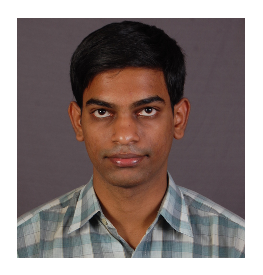
\includegraphics[width=1in,height=2.25in,clip,keepaspectratio]{sarvendranath.eps}}]{Rimalapudi Sarvendranth} (S'12)
	received his Bachelor of Technology degree in Electrical and Electronics Eng.\ from National Institute of Technology Karnataka, Surathkal in 2009. He received his Master of Eng.\ degree from the Dept.\ of Electrical Communication Eng.\, Indian Institute of Science (IISc), Bangalore in 2012. He is currently a Ph.D. student in the Dept.\ of  Electrical   Communication  Eng.\, IISc, Bangalore. From 2009--2010, he was a research assistant in the  Dept.\ of Instrumentation, IISc, Bangalore where he was involved in the  development of image processing algorithms. From 2012--2016, he was with Broadcom Communications Technologies Pvt.\ Ltd., Bangalore, India, where he worked on the development and implementation of algorithms for LTE and IEEE 802.11ac wireless standards.  His research interests include wireless communication, multiple antenna techniques, cognitive radio and next generation wireless standards.
\end{IEEEbiography}

\begin{IEEEbiography}[{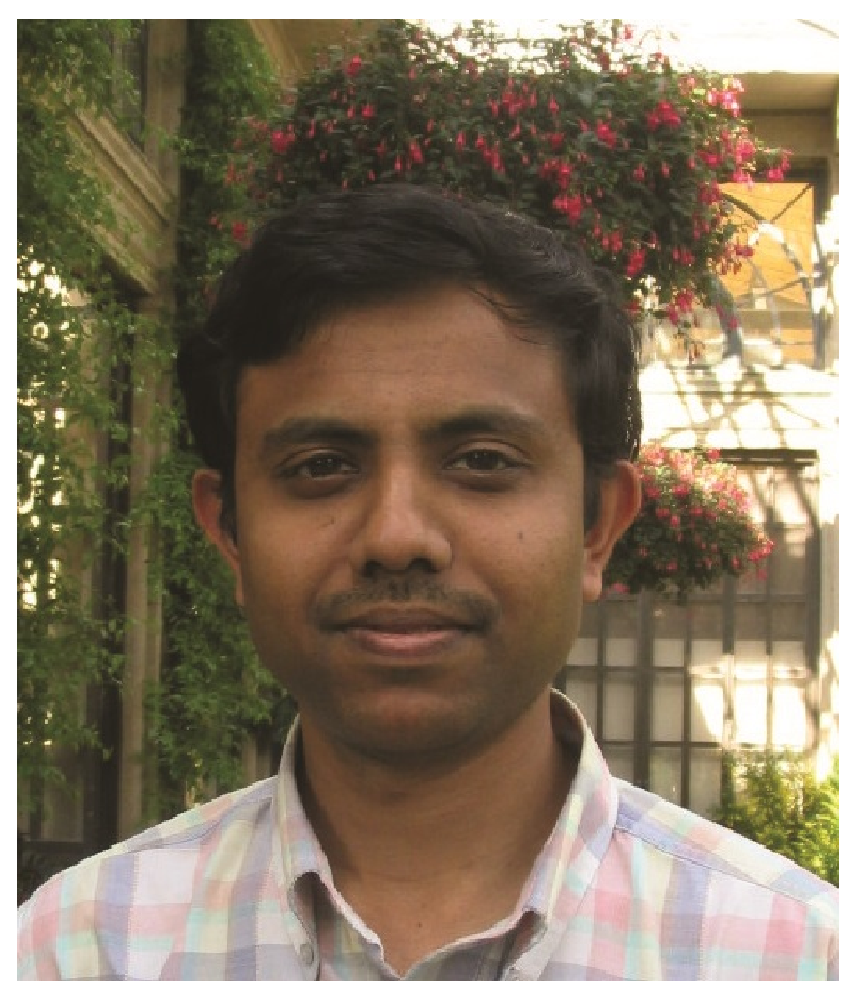
\includegraphics[width=1in,height=2.25in,clip,keepaspectratio]{neelesh_b_mehta}}]
	{Neelesh B. Mehta} (S'98-M'01-SM'06) received his Bachelor of Technology degree in Electronics and Communications Engineering from the Indian Institute of Technology (IIT), Madras in 1996, and his M.S. and Ph.D. degrees in Electrical Engineering from the California Institute of Technology, Pasadena, USA in 1997 and 2001, respectively. He is a Professor in the Department of Electrical Communication Engineering, Indian Institute of Science, Bangalore. He is a Fellow of the Indian National Academy of Engineering (INAE) and the National Academy of Sciences India (NASI). He is a recipient of the Shanti Swarup Bhatnagar Award 2017 and the Swarnjayanti Fellowship. He serves as the Chair of the Executive Editorial Committee of the IEEE Transactions on Wireless Communications, and as an Editor of the IEEE Transactions on Communications. He served on the Board of Governors of IEEE ComSoc from 2012 to 2015.
\end{IEEEbiography}


\end{document}


